\documentclass[12pt,a4paper,oneside]{report}
\usepackage[margin=2.4cm,left=3cm,headheight=16pt]{geometry}
\usepackage{fontspec}
\IfFontExistsTF{Times New Roman}{\setmainfont{Times New Roman}}{\setmainfont{TeX Gyre Termes}}
\IfFontExistsTF{Arial}{\setsansfont{Arial}}{\setsansfont{TeX Gyre Heros}}
\IfFontExistsTF{Consolas}{\setmonofont{Consolas}}{\setmonofont{Latin Modern Mono}}
\usepackage{amsmath,amssymb,graphicx,booktabs,tabularx,array,float}
\usepackage{caption,subcaption,setspace,fancyhdr,titlesec,xcolor,listings,enumitem}
\usepackage[unicode,colorlinks=true,linkcolor=black,citecolor=black,urlcolor=blue,bookmarksnumbered=true]{hyperref}
\usepackage{bookmark}
\usepackage[section]{placeins}
\renewcommand{\contentsname}{Mục lục}
\renewcommand{\listfigurename}{Danh mục hình}
\renewcommand{\listtablename}{Danh mục bảng}
\renewcommand{\figurename}{Hình}
\renewcommand{\tablename}{Bảng}
\renewcommand{\chaptername}{Chương}
\renewcommand{\bibname}{Tài liệu tham khảo}
\renewcommand{\appendixname}{Phụ lục}
\renewcommand{\lstlistingname}{Mã nguồn}
\setcounter{tocdepth}{1}
\setlength{\parindent}{1.1cm}\setlength{\parskip}{4pt}
\setstretch{1.12}
\emergencystretch=2em
\pagestyle{fancy}\fancyhf{}
\fancyhead[L]{\small PTIT -- Xử lý ảnh}\fancyhead[R]{\small Nhóm 1}
\fancyfoot[C]{\thepage}\renewcommand{\headrulewidth}{0.4pt}
\fancypagestyle{plain}{\fancyhf{}\fancyfoot[C]{\thepage}\renewcommand{\headrulewidth}{0pt}}
\titleformat{\chapter}[display]{\bfseries\Large}{\chaptername\ \thechapter}{8pt}{\LARGE}
\titlespacing*{\chapter}{0pt}{0pt}{18pt}
\titleformat{\section}{\large\bfseries}{\thesection}{0.7em}{}
\captionsetup{font=small,labelfont=bf,labelsep=period}
\lstset{language=Python,basicstyle=\ttfamily\scriptsize,breaklines=true,breakatwhitespace=false,numbers=left,numberstyle=\tiny\color{gray},frame=single,rulecolor=\color{gray!40},columns=fullflexible,keepspaces=true,showstringspaces=false,tabsize=4,captionpos=b}
\hypersetup{pdftitle={Phân đoạn đối tượng bằng hình thái học toán học và Watershed},pdfauthor={PTIT Nhóm 1}}
\begin{document}\hypersetup{pageanchor=false}
\begin{titlepage}\centering
{\large\bfseries HỌC VIỆN CÔNG NGHỆ BƯU CHÍNH VIỄN THÔNG}\par
\vspace{1cm}{\large BÁO CÁO BÀI TẬP LỚN}\par
\vspace{0.3cm}{\Large\bfseries MÔN XỬ LÝ ẢNH}\par
\vspace{1.2cm}\rule{\linewidth}{0.6pt}\par
\vspace{0.5cm}{\LARGE\bfseries PHÂN ĐOẠN ĐỐI TƯỢNG BẰNG\par HÌNH THÁI HỌC TOÁN HỌC\par VÀ WATERSHED}\par
\vspace{0.5cm}\rule{\linewidth}{0.6pt}\par
\vspace{0.8cm}{\large Nền tảng tham chiếu: Fiji/ImageJ -- MorphoLibJ}\par
\vspace{0.7cm}{\large\bfseries Nhóm 1}\par\vspace{0.4cm}
\begin{tabular}{ll}\toprule
\textbf{Họ và tên}&\textbf{Mã sinh viên}\\\midrule
Kiều Trường Giang&B23DCCN254\\
Trần Đỗ Lan Phương&B23DCCN667\\
Giang Thùy Tiên&B23DCCN814\\
Phạm Văn Vỹ&B23DCCN954\\\bottomrule
\end{tabular}
\vfill
\href{https://github.com/jellalaz/XU_LY_ANH}{github.com/jellalaz/XU\_LY\_ANH}\par
\vspace{0.5cm}Tháng 11 năm 2026
\end{titlepage}
\pagenumbering{roman}\hypersetup{pageanchor=true}
\chapter*{Tóm tắt}\addcontentsline{toc}{chapter}{Tóm tắt}
Nhóm xây dựng quy trình chuẩn hóa ảnh, tạo mặt nạ, xử lý hình thái, tính khoảng cách tới nền, tạo marker và lan nhãn bằng Watershed. Cài đặt tự viết tập trung ở các phép hình thái nhị phân, tái tạo, gán nhãn liên thông, khoảng cách Euclid và hàng đợi ưu tiên. Gaussian, Otsu, đọc ghi và thống kê sử dụng thư viện được công bố rõ.

Trên 50 ảnh test BBBC039, F1 trung bình theo ảnh của Python tự cài đạt 0,7087; Python thư viện đạt 0,7054; Fiji nhận chung đầu vào đạt 0,7188; quy trình Fiji độc lập đạt 0,8917. Các quy trình có tiền xử lý khác nhau, vì vậy số liệu này không chứng minh riêng một hàm Watershed luôn tốt hơn hàm khác. IoU tiền cảnh cao cũng chưa bảo đảm tách đúng từng vật thể.

Mục tiêu học thuật là giải thích được thuật toán, quy ước cài đặt, thiết kế kiểm chứng và nguyên nhân sai khác. Nhóm không huấn luyện mô hình học sâu. Kết quả là nghiên cứu phân đoạn hình thái, có giới hạn khi đối tượng không tách biệt về độ sáng hoặc hình dạng.


\clearpage\tableofcontents\clearpage\listoffigures\clearpage\listoftables\clearpage\pagenumbering{arabic}
\chapter{Giới thiệu và phạm vi nghiên cứu}\label{chap:intro}

\section{Bài toán và câu hỏi nghiên cứu}
Đầu vào là ảnh xám hai chiều I có H hàng và W cột. Nếu đầu vào RGB, chương trình chuyển thành ảnh xám trước khi xử lý. Đầu ra L là ảnh nhãn nguyên không âm cùng kích thước: 0 là nền, mỗi số dương nhận diện một đối tượng. Ảnh tô màu chỉ dùng quan sát; ảnh nhãn TIFF mới là dữ liệu để tính chỉ số.

Phân đoạn tiền cảnh trả lời pixel nào thuộc đối tượng. Phân đoạn từng đối tượng còn cần phân chia các pixel tiền cảnh thành những vật thể khác nhau. Hai nhân tế bào đang chạm nhau có thể tạo một vùng liên thông nhưng phải mang hai nhãn trong kết quả mong muốn. Đếm số nhãn là một phép đo sau phân đoạn, không phải toàn bộ bài toán.

Nghiên cứu đặt ra bốn câu hỏi: các toán tử tự cài có tuân thủ định nghĩa và quy ước biên không; Python và Fiji khác nhau thế nào khi nhận cùng đầu vào; hình thái và marker ảnh hưởng thế nào đến lỗi gộp hoặc chia; chi phí tính toán thay đổi ra sao giữa các cách cài đặt.

Phạm vi gồm đủ tám nội dung trong đề tài: erosion, dilation, opening, closing, morphological reconstruction, distance transform, watershed và connected components. Báo cáo trình bày từng phép và cách phối hợp trong quy trình hoàn chỉnh. Phân đoạn dựa trên độ sáng và hình dạng không gán tên ngữ nghĩa như người, xe hoặc động vật.


\begin{figure}[H]\centering
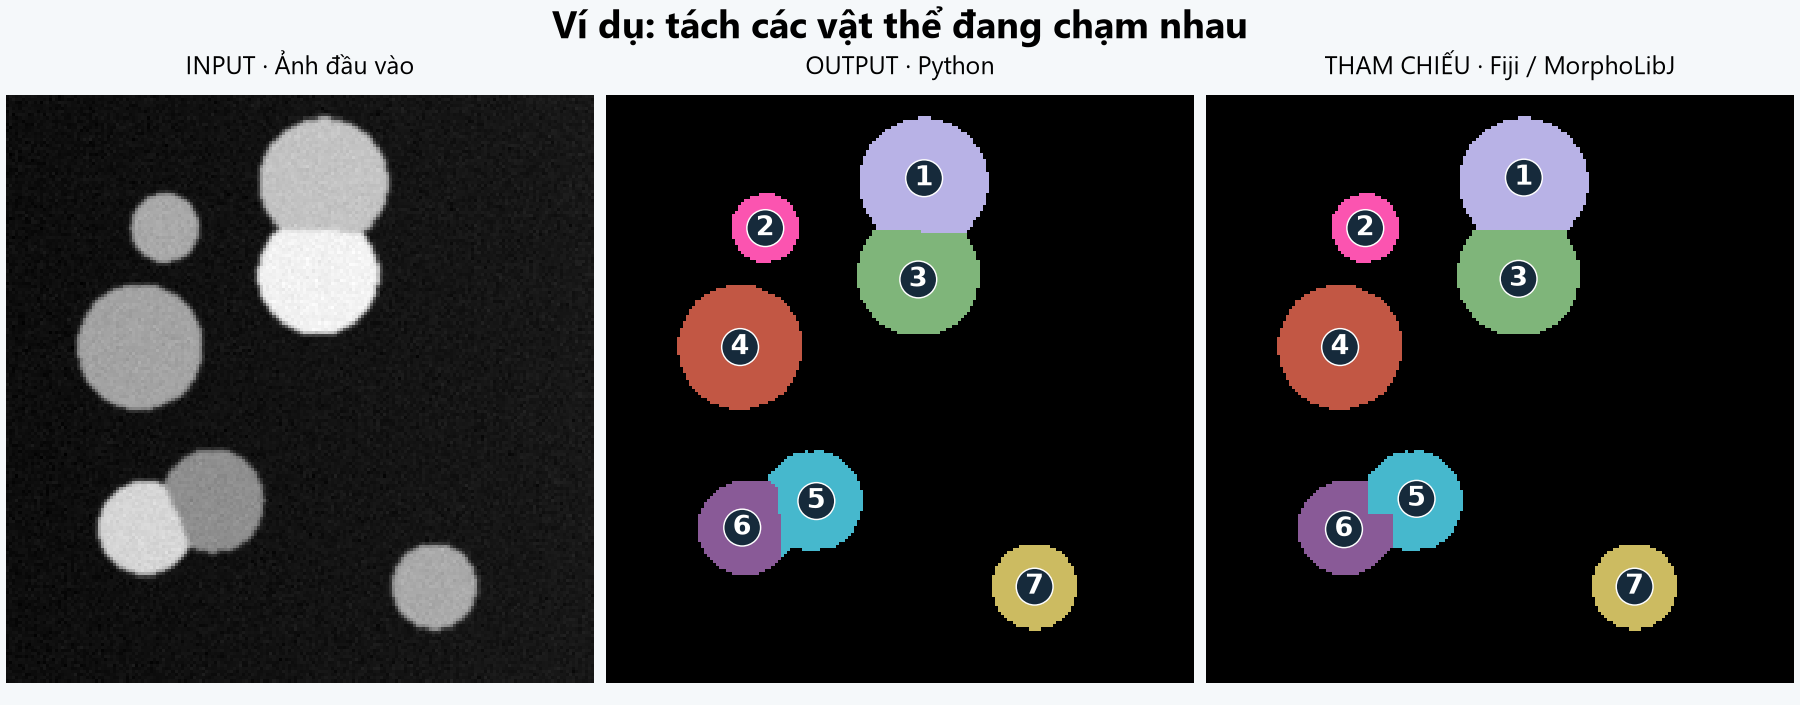
\includegraphics[width=\linewidth]{figures/input_output.png}
\caption{Ảnh đầu vào, nhãn Python và nhãn Fiji: ví dụ bảy vật thể có hai cặp chạm nhau.}\label{fig:example}
\end{figure}

\section{Mục tiêu và sản phẩm nghiên cứu}
Nhóm cung cấp lý thuyết, mã tự cài, kết quả Fiji và đánh giá định lượng. MorphoLab hỗ trợ thao tác.
\chapter{Cơ sở lý thuyết hình thái học và Watershed}\label{chap:theory}

\section{Biểu diễn ảnh và các quy ước toán học}
Với ảnh nhị phân, A là tập các tọa độ pixel tiền cảnh. Phần tử cấu trúc B là tập độ lệch quanh một gốc xác định. Chương trình dùng phần tử có kích thước lẻ 2r+1 để gốc nằm ở tâm. Ba hình dạng khảo sát là đĩa, vuông và chữ thập. Đĩa bán kính 1 trên lưới số nguyên có dạng chữ thập, khác hình vuông 3\ensuremath{\times}3.

Lân cận 4 gồm trên, dưới, trái, phải. Lân cận 8 bổ sung bốn đường chéo. Đây là tham số có ảnh hưởng đến số vùng, khả năng lan tái tạo và đường phân chia Watershed. Không được đổi liên thông giữa hai bản rồi xem chênh lệch là lỗi triển khai.

\begin{equation}\mathcal{N}_4(x,y)=\{(x-1,y),(x+1,y),(x,y-1),(x,y+1)\}\end{equation}
\begin{equation}\mathcal{N}_8(x,y)=\mathcal{N}_4(x,y)\cup\{(x\pm1,y\pm1)\}\end{equation}

Ngoài miền ảnh, phép hình thái nhị phân coi pixel là nền 0. Distance transform thêm một khung nền dày một pixel; quy ước này quyết định khoảng cách khi toàn ảnh là tiền cảnh. Trong tái tạo ảnh xám, giá trị ngoài miền là âm vô cùng khi tính giãn, để không tạo mức sáng mới ở biên.

Ảnh cường độ được chuẩn hóa min–max về [0,1]. Ảnh hằng được ánh xạ thành 0; đây là quy ước xác định, không suy diễn rằng một ảnh hằng chứa đối tượng. Ngưỡng thủ công sử dụng đơn vị đã chuẩn hóa, còn h trong bản dựa trên khoảng cách có đơn vị pixel. Diện tích được đo theo pixel\ensuremath{^2} do thí nghiệm chưa sử dụng kích thước vật lý của pixel.

\section{Erosion và Dilation}
Erosion, hay phép co, giữ vị trí x nếu toàn bộ phần tử B khi đặt tại x nằm trong A. Phép này làm vùng tiền cảnh nhỏ lại, có thể loại điểm lẻ hoặc phá cầu nối mảnh. Dilation, hay phép giãn, bổ sung các vị trí có thể đạt được bằng cách cộng một điểm của A với một độ lệch trong B. Nó làm vùng mở rộng và có thể nối hai vật thể vốn gần nhau.

\begin{equation}A\ominus B=\{x:x+B\subseteq A\}\end{equation}
\begin{equation}A\oplus B=\{a+b:a\in A,b\in B\}\end{equation}

Ở dạng phép toán pixel, erosion là AND các ảnh dịch theo x+b; dilation là OR các ảnh dịch theo x-b. Dấu của độ lệch quan trọng với phần tử bất đối xứng. Nếu chỉ thử phần tử vuông hoặc đĩa đối xứng, lỗi phản xạ có thể không bị phát hiện. Bộ kiểm thử có thêm phần tử bất đối xứng để kiểm tra trường hợp này.

Cài đặt không duyệt từng cửa sổ bằng Python: với mỗi điểm khác 0 của SE, lấy một lát của ảnh đã đệm, rồi AND hoặc OR trên toàn mảng NumPy. Nếu N=H\ensuremath{\times}W và k là số điểm của SE, số phép toán tỷ lệ O(Nk), bộ nhớ phụ tỷ lệ O(N) ngoài ảnh đệm. Đây là cách cài dễ đối chiếu với định nghĩa; SE lớn vẫn có thể tốn thời gian.

Ảnh xám có định nghĩa tổng quát bằng min/max trên lân cận với phần tử phẳng. Phần tự cài và đối chiếu ở dự án này dùng hình thái nhị phân trong quy trình phân đoạn; tái tạo ảnh xám được dùng khi lọc cực đại và cài đặt trong chương Python.

\section{Opening và Closing}
Opening là erosion rồi dilation với cùng phần tử cấu trúc. Closing là dilation rồi erosion. Opening thường loại vùng nhỏ không chứa được phần tử cấu trúc; closing thường khép khe nhỏ và lỗ nhỏ. Hai phép không phải hai phép nghịch đảo, vì thông tin bị loại có thể không khôi phục được.

\begin{equation}A\circ B=(A\ominus B)\oplus B\end{equation}
\begin{equation}A\bullet B=(A\oplus B)\ominus B\end{equation}

Trên miền vô hạn với quy ước phù hợp, opening có tính phản mở rộng và closing có tính mở rộng; cả hai là phép lũy đẳng. Trên miền hữu hạn với nền ngoài ảnh bằng 0 và cắt lại sau từng bước, cần thận trọng khi kiểm tra các tính chất tại biên. Báo cáo vì vậy nêu rõ quy ước đệm thay vì giả định mọi thư viện đều xử lý giống nhau.

Ví dụ với khối vuông 3\ensuremath{\times}3 nằm giữa ảnh 7\ensuremath{\times}7 và SE vuông 3\ensuremath{\times}3, co tạo một pixel trung tâm, giãn tạo khối 5\ensuremath{\times}5, opening khôi phục khối 3\ensuremath{\times}3 ban đầu. Nếu thêm một pixel rời xa khối, opening loại pixel đó. Nếu hai vật thể chỉ cách nhau một khe hẹp, closing có thể nối chúng và làm bài toán tách khó hơn.

Phần mềm có cả opening thường, closing và opening rồi closing. Mặc định của quy trình nghiên cứu là opening bằng reconstruction, nhằm loại vùng không còn hạt giống sau co nhưng khôi phục hình dạng của những vùng còn hạt giống. Không có lựa chọn nào được coi là tối ưu cho mọi ảnh; phép ablation đo tác dụng thực tế của từng bước.

\begin{figure}[H]\centering
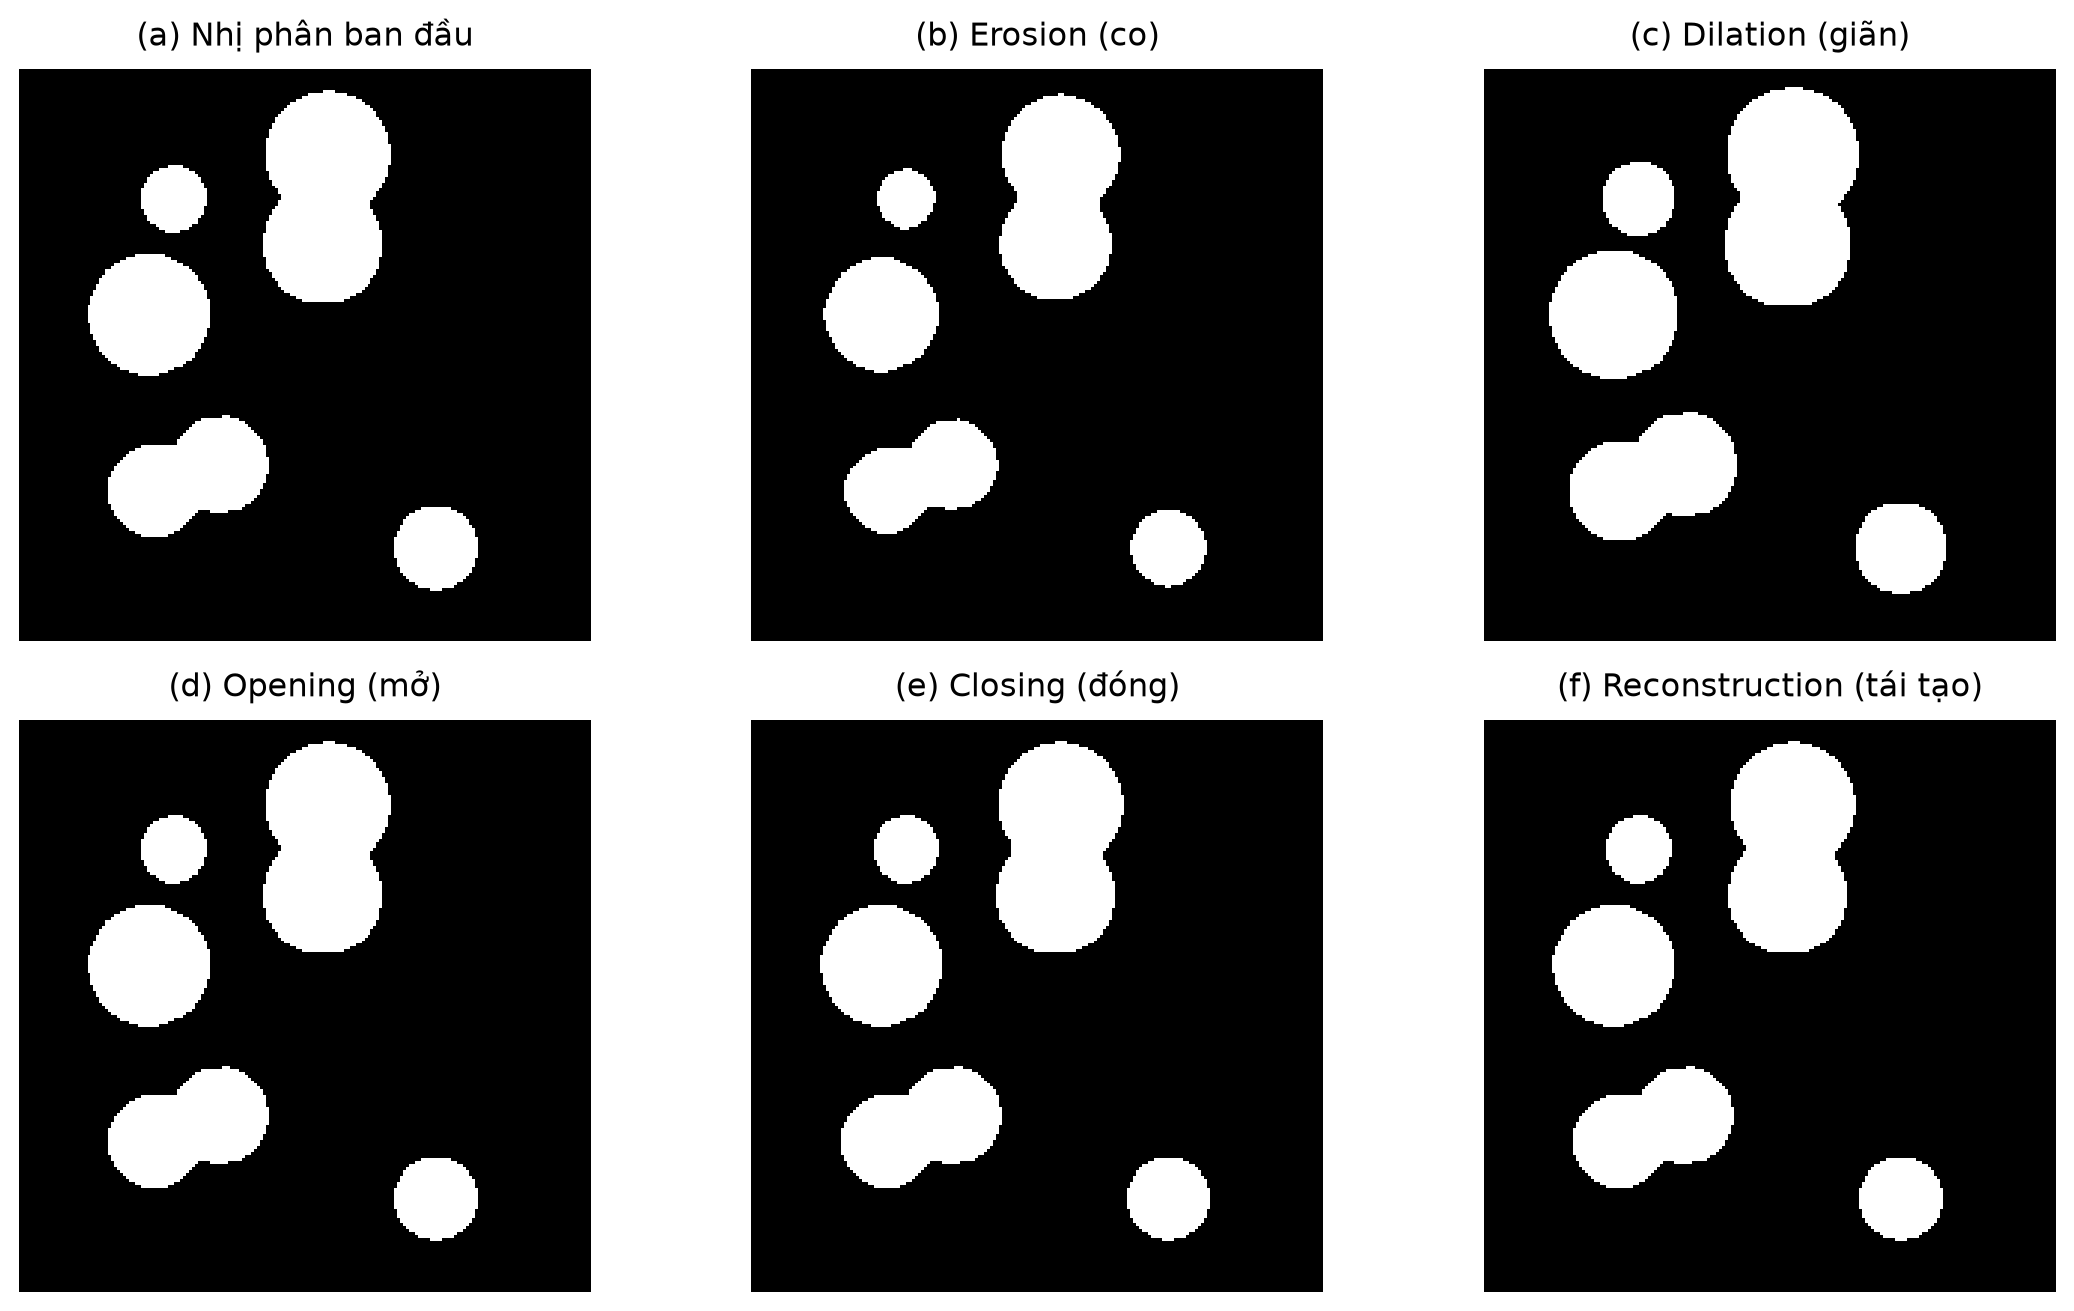
\includegraphics[width=\linewidth]{figures/morphology.png}
\caption{Các toán tử hình thái chạy thật bằng Fiji native, SE vuông bán kính 1.}\label{fig:morphology}
\end{figure}

\section{Ví dụ tính tay và kết quả kiểm tra}
Chọn A là khối 3\ensuremath{\times}3 tại hàng 2 đến 4 và cột 2 đến 4 của ảnh 7\ensuremath{\times}7, chỉ số bắt đầu từ 0. B là toàn bộ khối 3\ensuremath{\times}3 có gốc tại tâm. Tại tâm (3,3), B nằm hoàn toàn trong A nên erosion bằng 1. Tại (2,3), B chạm hàng 1 là nền nên erosion bằng 0. Dilation tại (1,3) bằng 1 vì một điểm của B dịch đến A; tại (0,3) vẫn bằng 0.

\begin{equation}\resizebox{0.92\linewidth}{!}{$ A=\begin{bmatrix}0&0&0&0&0&0&0\\0&0&0&0&0&0&0\\0&0&1&1&1&0&0\\0&0&1&1&1&0&0\\0&0&1&1&1&0&0\\0&0&0&0&0&0&0\\0&0&0&0&0&0&0\end{bmatrix}\quad A\ominus B=\begin{bmatrix}0&0&0&0&0&0&0\\0&0&0&0&0&0&0\\0&0&0&0&0&0&0\\0&0&0&1&0&0&0\\0&0&0&0&0&0&0\\0&0&0&0&0&0&0\\0&0&0&0&0&0&0\end{bmatrix}\quad A\oplus B=\begin{bmatrix}0&0&0&0&0&0&0\\0&1&1&1&1&1&0\\0&1&1&1&1&1&0\\0&1&1&1&1&1&0\\0&1&1&1&1&1&0\\0&1&1&1&1&1&0\\0&0&0&0&0&0&0\end{bmatrix}\quad $}\end{equation}

Các ma trận trên được tạo từ code đang nộp bằng scripts/academic\_checks.py và lưu ở docs/evidence/academic\_checks/hand\_examples.json. Có thể kiểm tra từng ô theo định nghĩa trước khi chạy lại script. Tổng số pixel tiền cảnh tương ứng của ảnh gốc, co và giãn là 9, 1 và 25. Hai phép opening và closing trả lại khối 3\ensuremath{\times}3 trong ví dụ ở giữa ảnh này.

Ví dụ nhỏ giúp kiểm tra quy ước tọa độ và dấu dịch. Nó không thay cho thí nghiệm ảnh thật vì không có nhiễu, độ sáng không đồng nhất hoặc hình dạng phức tạp. Trường hợp biên và SE bất đối xứng được kiểm tra thêm trong tests/test\_algorithms.py.

\section{Tái tạo hình thái}
Tái tạo bằng giãn nhận ảnh đánh dấu M và ảnh giới hạn F, cùng kích thước và thỏa M\ensuremath{\leq}F. Bắt đầu từ X0=M, mỗi bước giãn X rồi lấy min với F. Dãy tăng đơn điệu nhưng không vượt F. Trên ảnh số hữu hạn, quá trình đạt điểm bất động. Với ảnh nhị phân, min tương đương giao tập.

\begin{equation}X_0=M,\quad X_{k+1}=\min(\delta(X_k),F),\quad R_F^\delta(M)=X_k\ \text{khi }X_{k+1}=X_k\end{equation}

Phân biệt hai khái niệm marker: ảnh đánh dấu của reconstruction là cường độ ban đầu cho lan truyền; marker của Watershed là ảnh nhãn các vùng khởi tạo. Chúng có vai trò khác nhau dù cùng tên tiếng Anh. Mặt nạ reconstruction giới hạn giá trị cường độ, còn mask nhị phân của Watershed giới hạn miền được gán nhãn.

Opening by reconstruction lấy M là ảnh sau erosion và F là ảnh nhị phân trước co. Vùng nào mất hết hạt giống sẽ biến mất; vùng còn ít nhất một hạt giống sẽ lan lại bên trong F. Cách này có thể giữ hình dạng vùng tốt hơn opening thường, nhưng cũng khôi phục cầu nối khiến hai vật thể vẫn liên thông. Vì vậy cần Watershed ở bước sau nếu muốn tách vật thể chạm nhau.

Lấp lỗ bằng reconstruction thực hiện trên phần bù: dùng nền ở biên ảnh làm hạt giống, lan trong nền, sau đó lấy phần bù của phần nền tiếp cận được. Nền không nối tới biên trở thành lỗ được lấp. Lựa chọn liên thông ảnh hưởng đến việc một đường chéo mảnh có thông ra ngoài hay không.

\section{Gán nhãn các vùng liên thông}
Connected components labeling, viết tắt CCL, gán cùng một nhãn cho những pixel tiền cảnh có đường đi qua các pixel tiền cảnh theo liên thông đã chọn. Chương trình quét các pixel tiền cảnh; khi gặp điểm chưa có nhãn, tạo nhãn mới và duyệt BFS bằng hàng đợi để lan trong vùng đó.

\begin{equation}L(p)=L(q)\quad\text{nếu }p,q\text{ thuộc cùng thành phần liên thông của mask}\end{equation}

Mỗi pixel được gán nhãn tối đa một lần, mỗi điểm kiểm tra tối đa 4 hoặc 8 láng giềng. Độ phức tạp O(N), bộ nhớ O(N) cho ảnh nhãn và hàng đợi. Giá trị nhãn chỉ là mã định danh: kết quả [1,2] và [8,3] có thể biểu diễn cùng một phân đoạn. Không được so sánh trực tiếp màu tô hoặc ID để kết luận khác biệt thuật toán.

Ví dụ ảnh đường chéo 3\ensuremath{\times}3 có ba pixel 1: liên thông 4 tạo ba vùng, liên thông 8 tạo một vùng. Ví dụ ảnh tổng hợp bảy vật thể có hai cặp chạm nhau: CCL có thể chỉ trả về năm vùng vì mỗi cặp nối nhau thành một thành phần.

Trong pipeline, CCL dùng để loại vùng dưới diện tích tối thiểu, tìm vùng chưa có marker và gán nhãn cho các cực đại. Nó cũng là baseline độc lập để đánh giá xem Watershed có thực sự cải thiện kết quả hay đang chia quá nhiều. Khi dữ liệu có nhiều vật thể đã tách rời, baseline đơn giản này có thể đạt F1 cao.



\section{Biến đổi khoảng cách Euclid}
Với mask A, distance transform trả khoảng cách từ mỗi điểm tiền cảnh tới nền gần nhất. Pixel nền có khoảng cách 0. Ở vật thể gần tròn, các điểm gần tâm thường có khoảng cách lớn; do đó các cực đại của ảnh khoảng cách là ứng viên marker.

\begin{equation}D(p)=\min_{q\notin A}\lVert p-q\rVert_2\end{equation}
\begin{equation}D^2(x,y)=\min_{(u,v)\text{ là nền}}\big((x-u)^2+(y-v)^2\big)\end{equation}

Tính khoảng cách tới mọi pixel nền một cách trực tiếp có chi phí lớn. Bản tự cài sử dụng thuật toán tách trục của Felzenszwalb và Huttenlocher \cite{ref3}: đặt f=0 ở nền và f=+\ensuremath{\infty} ở tiền cảnh, tính biến đổi một chiều theo cột rồi theo hàng. Với mỗi chiều, tìm bao dưới của các parabol (x-i)\ensuremath{^2}+f(i). Các điểm giao quyết định khoảng chỉ số mà mỗi parabol nhỏ nhất.

Mỗi parabol được thêm và loại khỏi bao hữu hạn lần, nên biến đổi một chiều có chi phí tuyến tính theo độ dài. Hai lượt toàn ảnh cho O(HW), rồi lấy căn bậc hai. Triển khai bỏ qua các vị trí có chi phí vô cùng và thêm khung nền một pixel để trường hợp toàn tiền cảnh vẫn hữu hạn.

Khoảng cách Euclid chính xác, chamfer và ImageJ EDM có thể có sai khác. Khi đối chiếu riêng Watershed, dự án dùng chung ảnh elevation float32 thay vì giả định các hàm distance transform của hai nền tảng giống hệt nhau. Khi chạy Fiji độc lập, khác biệt về distance map được ghi là một phần của khác biệt quy trình.

\section{Marker và lọc cực đại theo h}
Nếu lấy mọi cực đại địa phương làm marker, nhiễu hoặc gồ ghề nhỏ trên distance map có thể tạo quá nhiều hạt giống. Watershed sẽ chia một đối tượng thật thành nhiều mảnh. H-maxima giảm ảnh hưởng của cực đại có độ nổi thấp bằng reconstruction ảnh xám.

\begin{equation}R=R_D^\delta(D-h),\quad H_h=\{p:D(p)-R(p)\geq h\}\end{equation}

Trong code, ngưỡng so sánh có dung sai 10\ensuremath{^-}\ensuremath{^9} để hạn chế sai số dấu phẩy động. Ảnh kết quả cực đại được giao với mask và gán nhãn liên thông. Nếu một thành phần tiền cảnh không có marker, chương trình bổ sung một marker tại vị trí có khoảng cách lớn nhất trong thành phần đó. Quy tắc dự phòng ngăn vật thể bị bỏ trắng khi h quá cao, nhưng có thể gộp toàn thành phần vào một vật thể.

Bốn phương án được so sánh là CCL, raw marker, hmax và adaptive. Raw lấy cực đại chưa lọc. Hmax dùng h cố định. Adaptive sử dụng h riêng cho thành phần: max(h, \ensuremath{\alpha}\ensuremath{\times}Dmax). Đây là một giả thuyết cải tiến để thích ứng kích thước, chưa phải bảo đảm tăng độ chính xác.

Tăng h thường giảm marker và giảm chia thừa, nhưng tăng nguy cơ gộp vật thể. Giảm h có thể tách được nhiều tâm sát nhau nhưng nhạy với nhiễu. Khảo sát chọn h phải dùng validation; sau khi xem test không được tiếp tục sửa h rồi coi số liệu test mới là đánh giá độc lập.

\section{Watershed có điều khiển marker}
Watershed xem ảnh cường độ như địa hình và lan các nhãn từ điểm khởi tạo. Trong bài toán này, elevation E=-D khiến các vùng sâu trong vật thể trở thành vùng thấp. Mask ngăn nhãn lan ra nền. Mỗi marker mang một nhãn, các pixel chưa gán nhận nhãn trong quá trình lan.

Hàng đợi ưu tiên của bản tự cài sắp theo cặp (mức ngập, thứ tự đến). Khi mở rộng từ p tới q, mức ngập mới bằng max(mức hiện tại, E[q]). Các pixel marker giữ nguyên nhãn. Pixel được đưa vào hàng đợi khi gặp lần đầu; thứ tự đến quyết định tranh chấp ở vùng có cùng mức ưu tiên. Bản này không tạo đường phân cách nền, gọi là không tạo dams.

\begin{equation}\operatorname{cost}(q)=\max(\operatorname{cost}(p),E(q))\end{equation}

Quy tắc này tạo đầu ra xác định với thứ tự duyệt và liên thông cố định. Tuy nhiên một thư viện khác có thể xử lý plateau, thứ tự khởi tạo, khoảng cách trên vùng phẳng hoặc đường phân cách khác. Đó là lý do Fiji shared có thể khác ranh giới dù cùng mask và marker. Báo cáo không dùng tuyên bố tương đương tuyệt đối giữa mọi biến thể Watershed.

Với heap nhị phân và mỗi pixel được đưa vào tối đa một lần, chi phí chính O(N log N), bộ nhớ O(N). Tính đúng cơ bản được kiểm tra bằng các bất biến: nhãn ngoài mask bằng 0; nhãn marker được bảo toàn; thành phần có marker nhận nhãn. Chất lượng so với đối tượng thật cần đánh giá bằng ground truth riêng.
\chapter{Thực hành từng bước trên Fiji/ImageJ}\label{chap:fiji}
\section{Dữ liệu, mục tiêu và nhật ký thực hành}
Fiji/ImageJ và MorphoLibJ 1.6.5 được dùng như nền tảng tham chiếu \cite{ref1,ref2}. Phần này đi từ ảnh gốc đến ảnh nhãn bằng menu Fiji, không cần mở MorphoLab hoặc dùng Python tạo trước các đầu vào Watershed. Sau khi làm bằng tay, nhóm mới dùng code chấm và đối chiếu ở Chương~\ref{chap:implementation}. Script tự động giúp lặp lại thí nghiệm sau khi đã hiểu các bước.

Ảnh đầu vào \path{synth_00.tif} có kích thước $192\times192$, một kênh, 16-bit; min/max dữ liệu là 2749 và 64456. Có bảy vật thể, gồm hai cặp chạm nhau. \path{synth_00_gt.tif} chứa ID nhãn đúng 1--7 và nền 0, chỉ dùng đánh giá sau phân đoạn. Nhãn đúng không tham gia chọn marker hay tạo dự đoán.

Các TIFF tại \path{docs/evidence/fiji_manual} và ảnh chụp giao diện là dữ liệu người học đã lưu/gửi trong lần thực hành. Bán kính các ảnh học thử không đồng nhất: đối chiếu mảng xác nhận co r=1, giãn r=3, mở/đóng r=2, seed tái tạo từ co r=4. Vì thế hình toán tử ở đây minh họa thao tác, không dùng để kết luận riêng một phép tốt hơn phép khác. Hình~\ref{fig:morphology} ở chương lý thuyết mới là bộ cùng SE/radius=1. Nhật ký dữ liệu và hash được lưu trong \path{verification.json}.

\section{Bước 1--3: mở ảnh, chuẩn hóa và phân ngưỡng}
\begin{enumerate}[leftmargin=*,itemsep=3pt]
\item Mở \path{C:/Tools/Fiji/fiji-windows-x64.exe}; kiểm tra \textbf{Plugins $\to$ MorphoLibJ}. Chọn \textbf{File $\to$ Open}, mở ảnh gốc; \textbf{Image $\to$ Duplicate} để giữ nguyên dữ liệu nguồn.
\item Với bản sao, đặt khoảng Brightness/Contrast theo min/max thật, bật \textbf{Scale When Converting} trong \textbf{Edit $\to$ Options $\to$ Conversions}, rồi \textbf{Image $\to$ Type $\to$ 8-bit}. 2749 được ánh xạ về 0, 64456 về 255. Đây là lượng tử hóa có mất thông tin, không phải điều kiện bắt buộc của Watershed.
\item Nhân bản ảnh 8-bit; \textbf{Process $\to$ Filters $\to$ Gaussian Blur}, sigma=1. Lưu ảnh trước/sau để thấy làm trơn và ảnh hưởng lên biên.
\item Chọn \textbf{Image $\to$ Adjust $\to$ Threshold}: Otsu, Dark background bật, Red, không dùng stack. \textbf{Auto} tính ngưỡng theo phương pháp đã chọn; vùng đỏ chỉ là preview. Kiểm tra \textbf{Process $\to$ Binary $\to$ Options}: Black background bật; bấm \textbf{Apply} tạo mask vật 255/nền 0.
\end{enumerate}
Không chạy Auto Threshold nối tiếp trên mask đã nhị phân. Plugin Auto Threshold là một giao diện khác cho bài toán chọn ngưỡng; với 16-bit, cách dùng histogram có thể khác. Trong bước này việc chuyển 8-bit được ghi rõ để tái lập. Hình~\ref{fig:manual-preprocess} lấy trực tiếp từ TIFF lưu khi làm tay.
\begin{figure}[htbp]\centering
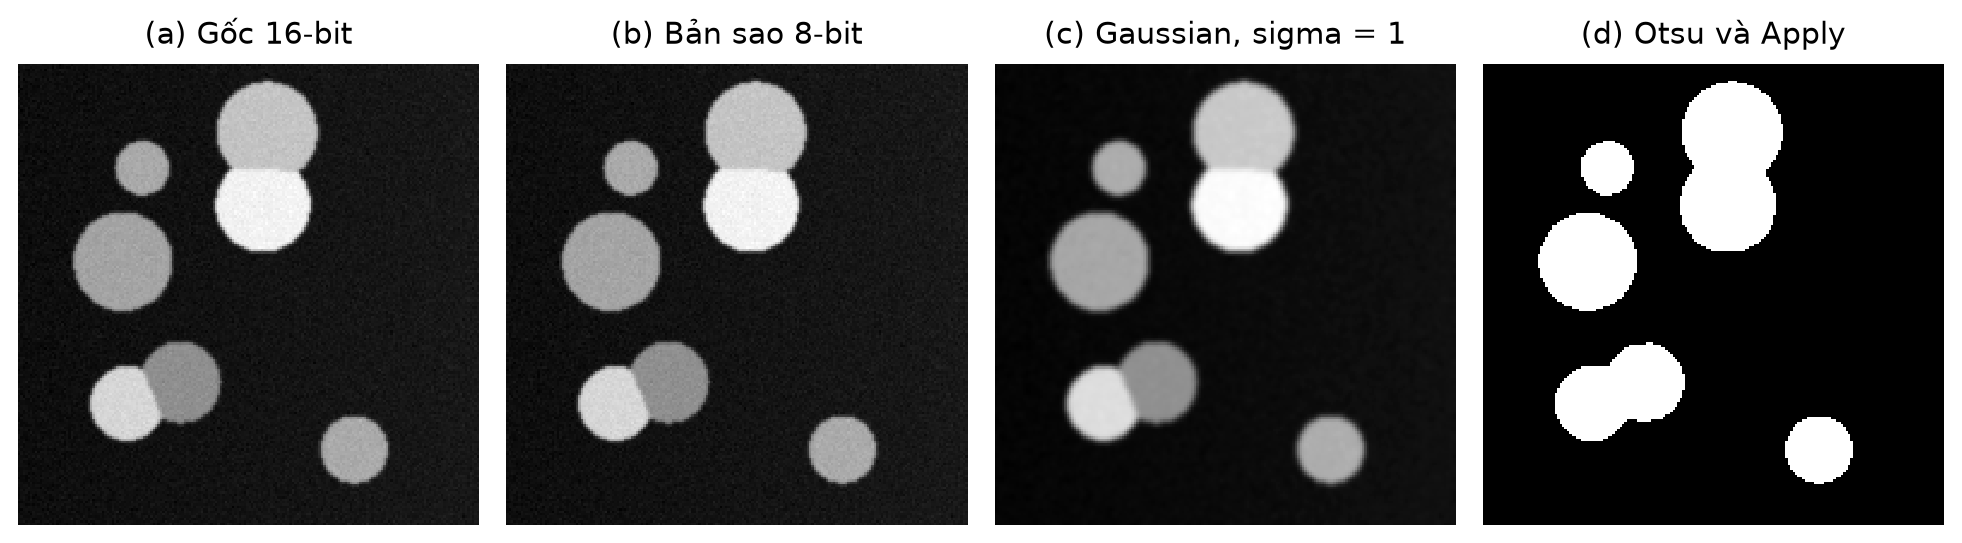
\includegraphics[width=\linewidth]{figures/manual_preprocess.png}
\caption{Ảnh thật của từng bước thực hành: nguồn 16-bit, bản sao 8-bit, Gaussian và nhị phân Otsu. Giống nhau về cách nhìn không có nghĩa dữ liệu không đổi.}\label{fig:manual-preprocess}
\end{figure}

\section{Bước 4: khảo sát co, giãn, mở, đóng và tái tạo}
Từ \emph{các bản sao độc lập của binary}, mở \textbf{MorphoLibJ $\to$ Filtering $\to$ Morphological Filters}. Operation chọn phép toán; Element chọn hình SE; Radius chọn tầm lân cận. Square r=4 có cạnh $2r+1=9$, không phải 4 pixel. Mỗi cửa sổ tính \emph{một} pixel đầu ra: co lấy MIN, giãn lấy MAX trên các vị trí được SE chọn; không giảm kích thước ảnh.

Opening co rồi giãn, loại chi tiết trắng nhỏ; Closing giãn rồi co, khép khe hoặc lỗ tối nhỏ. Mở không tạo thêm tiền cảnh ngoài ảnh gốc; đóng có thể nối vật gần nhau. Radius lớn dễ nhìn tác dụng nhưng cũng dễ làm mất vật thật. Các ảnh học thử trong Hình~\ref{fig:manual-morphology} ghi rõ bán kính khác nhau.
\begin{figure}[htbp]\centering
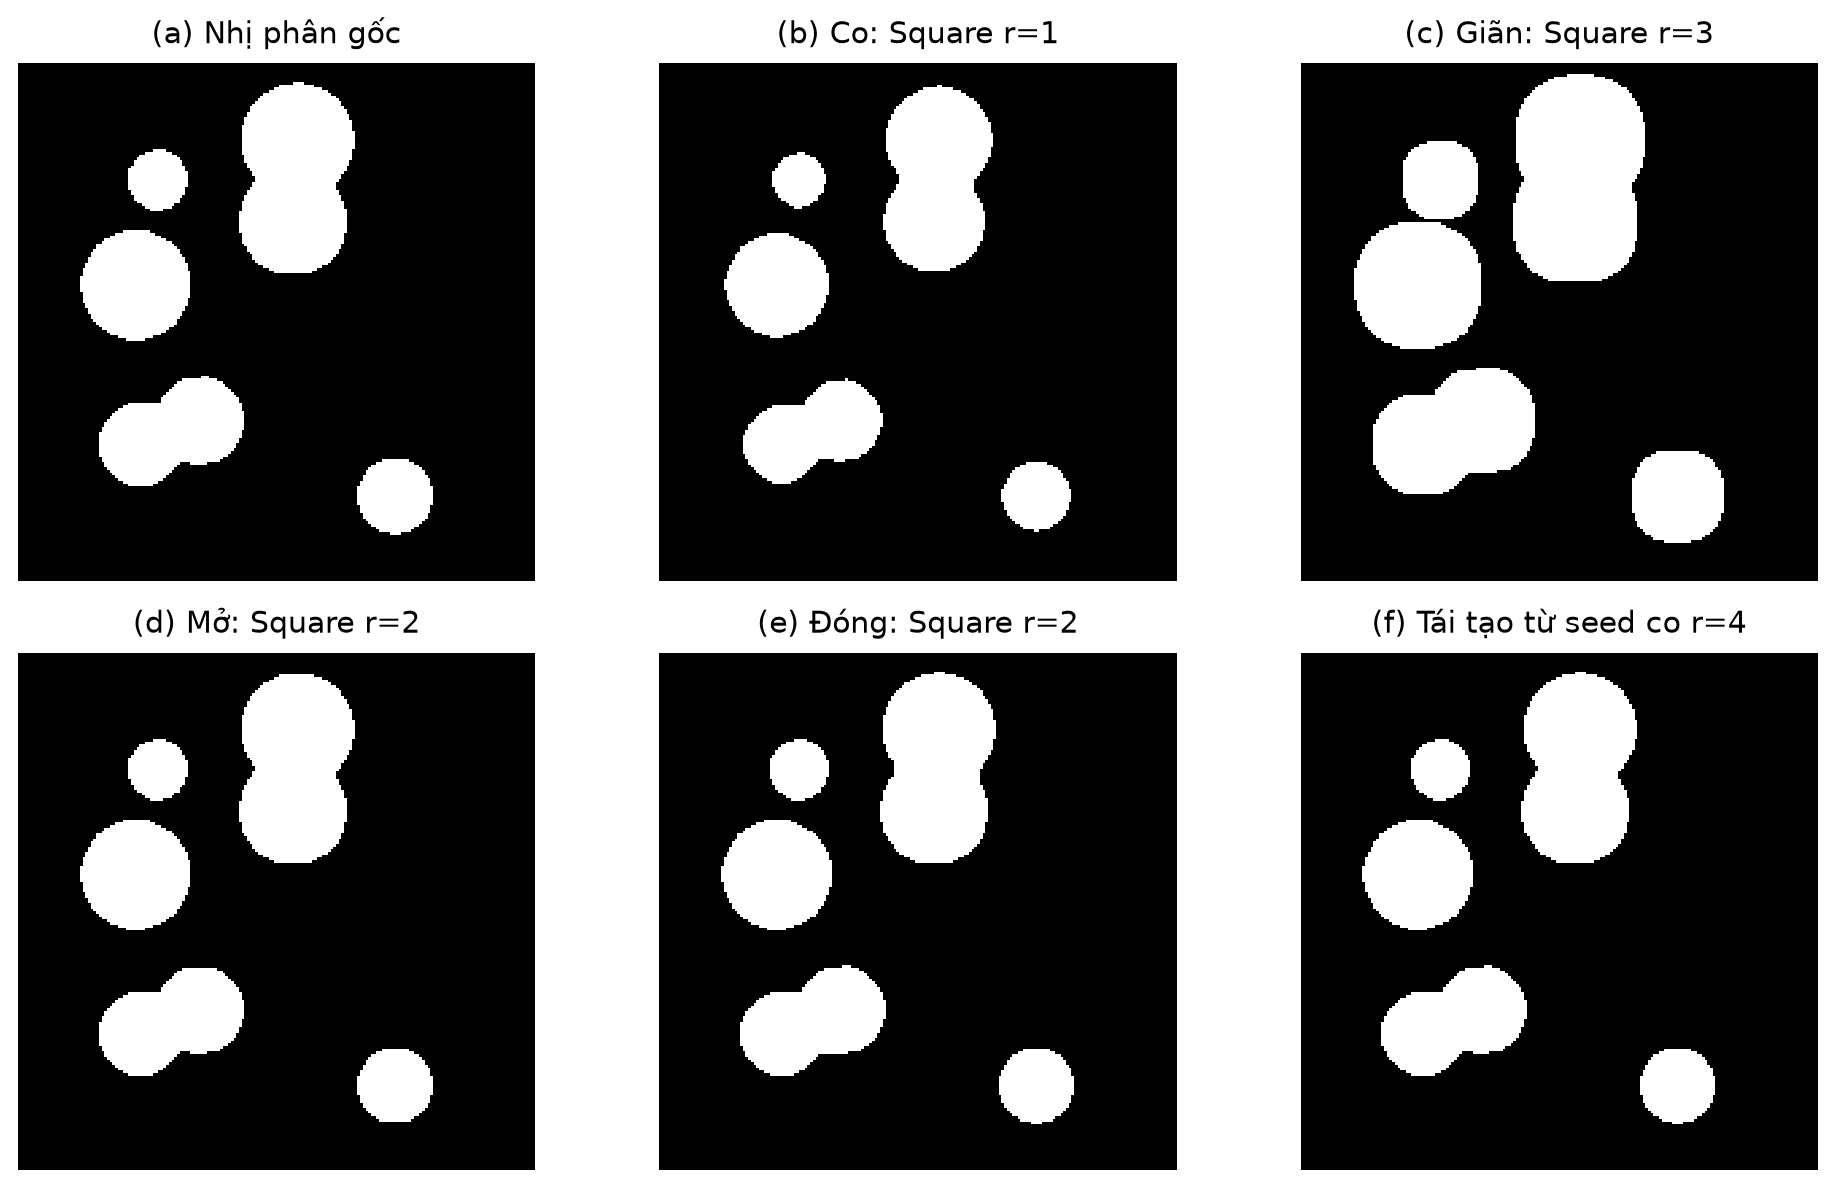
\includegraphics[width=\linewidth]{figures/manual_morphology.png}
\caption{Các kết quả Fiji do người học thực hiện. Đây là khảo sát thao tác với bán kính ghi trên từng ô; bộ so sánh cùng bán kính nằm ở Hình~\ref{fig:morphology}.}\label{fig:manual-morphology}
\end{figure}

Để mở bằng tái tạo, co binary thành seed, rồi gọi \textbf{Filtering $\to$ Morphological Reconstruction}: Marker Image=seed đã co, Mask Image=binary gốc, Type=By Dilation, Connectivity=4. Phép giãn bị mask chặn và lặp tới ổn định. Vùng liên thông còn ít nhất một seed được khôi phục; vùng mất seed hoàn toàn bị loại. Marker của tái tạo là ảnh khởi tạo cường độ, khác ảnh ID marker cho Watershed ở bước sau.

\section{Bước 5--6: làm sạch mask và đếm vùng liên thông}
Trên kết quả tái tạo, \textbf{Filtering $\to$ Fill Holes (Binary/Gray)} lấp nền kín bên trong vật. Nó không lấp khoảng trống thông ra nền ngoài. Sau đó \textbf{Binary Images $\to$ Size Opening 2D/3D}, Min Pixel Number=25, loại vùng liên thông nhỏ hơn 25 pixel, giữ nguyên hình dạng vùng còn lại. Hai vật dính nhau được tính chung diện tích. Lưu kết quả thành mask; nếu ảnh sạch, các bước này có thể không thay đổi pixel.

Chọn mask, \textbf{Binary Images $\to$ Connected Components Labeling}: Connectivity=4, Type=float. Đầu ra có năm ID vì mỗi cặp đang chạm nhau vẫn là một vùng. Chọn ảnh nhãn, \textbf{Analyze $\to$ Analyze Regions}, tích Area, Bounding Box, Centroid. Các ô tích chỉ yêu cầu tính cột, không lọc hoặc xóa vật. Area là diện tích, Centroid là trung bình tọa độ pixel, Bounding Box là hộp bao; gốc tọa độ ở góc trên trái, x tăng sang phải, y tăng xuống dưới.
\begin{figure}[htbp]\centering
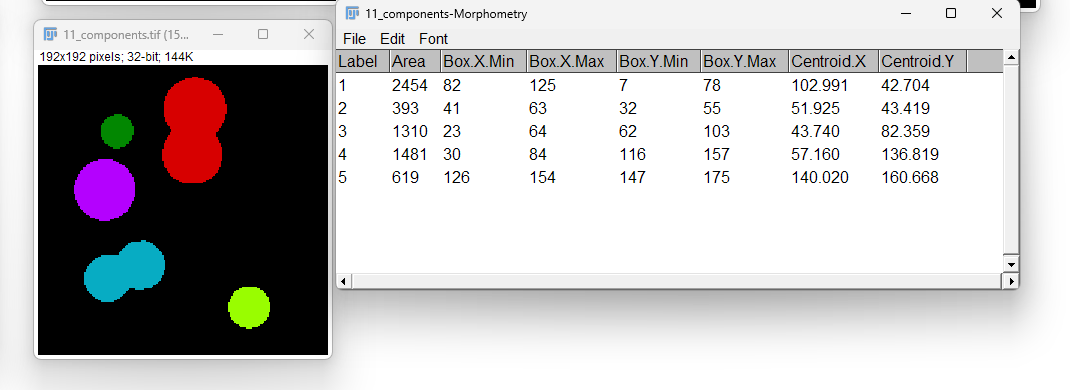
\includegraphics[width=0.94\linewidth]{figures/ui_components.png}
\caption{Ảnh chụp Fiji trong lần thực hành: năm vùng liên thông và bảng đo. Vùng đỏ gộp hai vật phía trên; vùng xanh ngọc gộp hai vật phía dưới.}\label{fig:manual-components}
\end{figure}

\section{Bước 7--8: distance, cực đại và marker có ID}
\begin{enumerate}[leftmargin=*,itemsep=3pt]
\item Chọn lại \emph{mask nhị phân 8-bit 0/255}, không chọn components. \textbf{Process $\to$ Binary $\to$ Options}: EDM output=32-bit; chạy \textbf{Distance Map}. Mỗi pixel trong vật nhận khoảng cách Euclid tới nền gần nhất. Đầu ra cần float để giữ khoảng cách lẻ; không chuyển distance 8-bit sang float sau khi đã mất độ chính xác.
\item Chọn distance 32-bit; \textbf{MorphoLibJ $\to$ Minima and Maxima $\to$ Extended Min \& Max}: \textbf{Extended Maxima}, Dynamic=2, Connectivity=4. h lọc độ nổi của cực đại, không phải số đối tượng hay ngưỡng cường độ tuyệt đối. Minima sẽ tìm vùng thấp, gồm nền, nên không dùng cho bước này.
\item Chọn \emph{ảnh kết quả mới của plugin}, là mask cực đại 8-bit. Không gán nhãn lên bản sao distance còn 32-bit. Kiểm tra ngoài cực đại=0, cực đại=255; Inverting LUT có thể làm màu nhìn ngược giá trị.
\item Chạy Connected Components Labeling trên mask cực đại: Connectivity=4, Type=float. Kết quả có bảy ID marker; một marker có thể gồm nhiều pixel. Không chỉnh marker theo ground truth để ép số lượng mong muốn.
\end{enumerate}
\begin{figure}[htbp]\centering
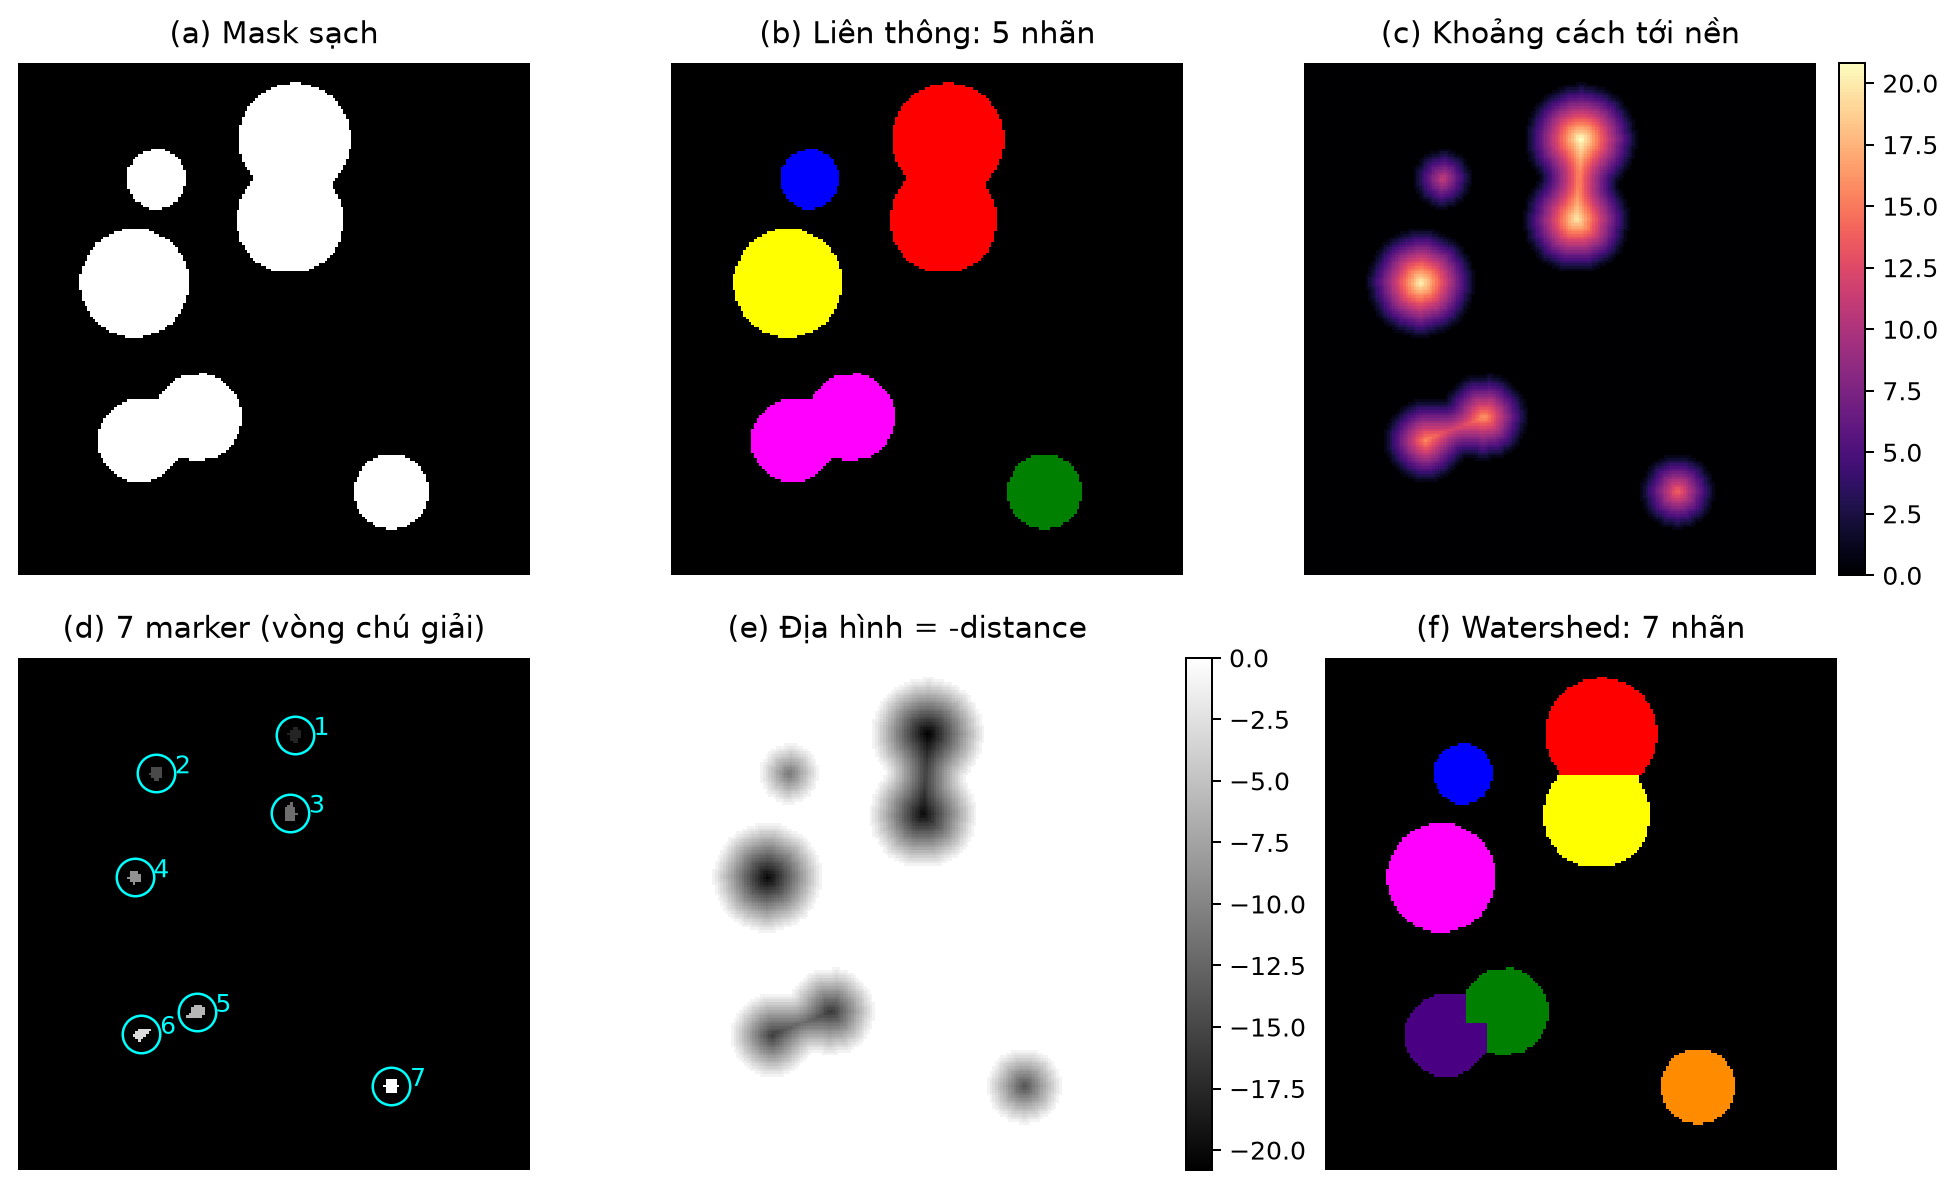
\includegraphics[width=\linewidth]{figures/manual_watershed.png}
\caption{Chuỗi dữ liệu thực hành: mask, năm thành phần, distance float, bảy marker, địa hình âm và nhãn Watershed. Vòng xanh ở ô marker chỉ chú giải vị trí, không thay kích thước seed trong TIFF.}\label{fig:manual-watershed}
\end{figure}

\section{Bước 9: địa hình âm và Marker-controlled Watershed}
Nhân bản distance, \textbf{Process $\to$ Math $\to$ Multiply}, nhập $-1$, nhận $E=-D$. Nền bằng 0, trong vật âm; tâm sâu hơn là vùng thấp. Chỉnh Brightness/Contrast chỉ để nhìn; Invert LUT không thay thế phép nhân.

Trong nhóm \textbf{MorphoLibJ $\to$ Segmentation}, mở lệnh \textbf{Marker-controlled Watershed}. Chọn Input là elevation, Marker là ảnh bảy ID và Mask là mặt nạ sạch. Đặt Compactness=0; bỏ Binary markers, Calculate dams và Use diagonal connectivity. Nhãn marker giữ ID riêng, không tạo đường nền phân cách, liên thông 4. Kết quả có bảy nhãn, được đo lại bằng Analyze Regions. Nhãn khác màu không có nghĩa khác vật; Spectrum từng làm nền và một nhãn trùng màu, nhưng bảng vẫn đủ bảy ID. LUT chỉ đổi cách hiển thị.

Kiểm tra tệp lưu phát hiện \path{15_elevation.tif} còn là bản distance dương trước phép nhân. Nhóm giữ nguyên bản này để truy vết và xuất lại $E=-D$ trong bộ minh chứng. Chạy lại MorphoLibJ trên $-D$ với marker/mask đã lưu cho nhãn trùng kết quả làm tay sau ghép ID, không pixel bất đồng; dùng $+D$ lệch 1915 pixel. Vì vậy báo cáo dùng địa hình âm đã kiểm chứng, không chỉ dựa vào tên tệp. Nhãn dự đoán làm tay không bị thay thế.

\section{Bước 10: đo IoU/Dice ngay trong Fiji}
Mở nhãn đúng; Duplicate cả nhãn đúng và nhãn dự đoán. Trên hai bản sao, tắt \textbf{Scale When Converting}, chuyển 8-bit để giữ nguyên ID nhỏ 0--7; Threshold $\to$ Set chọn 1--7, Apply thành vật 255/nền 0. Không dùng Otsu trên ID nhãn. Giữ nguyên hai TIFF nhãn gốc để đánh giá từng đối tượng bằng Python.

Trong nhóm \textbf{Analyze}, chọn \textbf{Label Overlap Measures}. Source là GT foreground, Target là Prediction foreground; bật Jaccard index và Dice coefficient. Vì mask chỉ còn nhãn tiền cảnh 255, bảng all-labels và individual-labels cho cùng số. Label 255 không phải 255 vật. Phép đo này đánh giá vật/nền, không tự chấm lỗi tách từng vật đang dính.
\begin{figure}[htbp]\centering
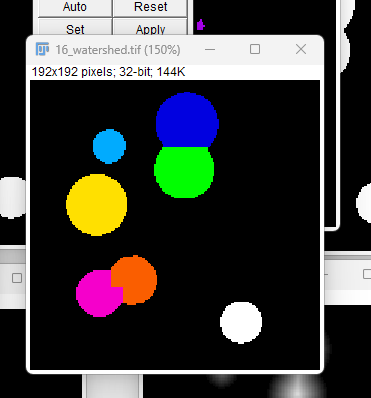
\includegraphics[width=0.28\linewidth]{figures/ui_watershed.png}\hfill
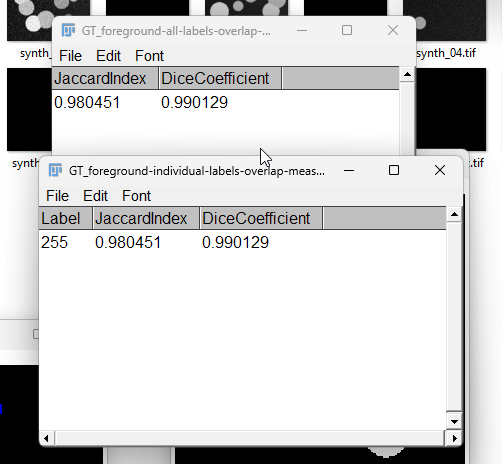
\includegraphics[width=0.66\linewidth]{figures/ui_overlap.png}
\caption{Ảnh chụp kết quả làm tay: nhãn Watershed hiển thị màu và bảng overlap Fiji, Jaccard=0,980451; Dice=0,990129. Các màu chỉ là LUT.}\label{fig:manual-ui-result}
\end{figure}

\begin{figure}[htbp]\centering
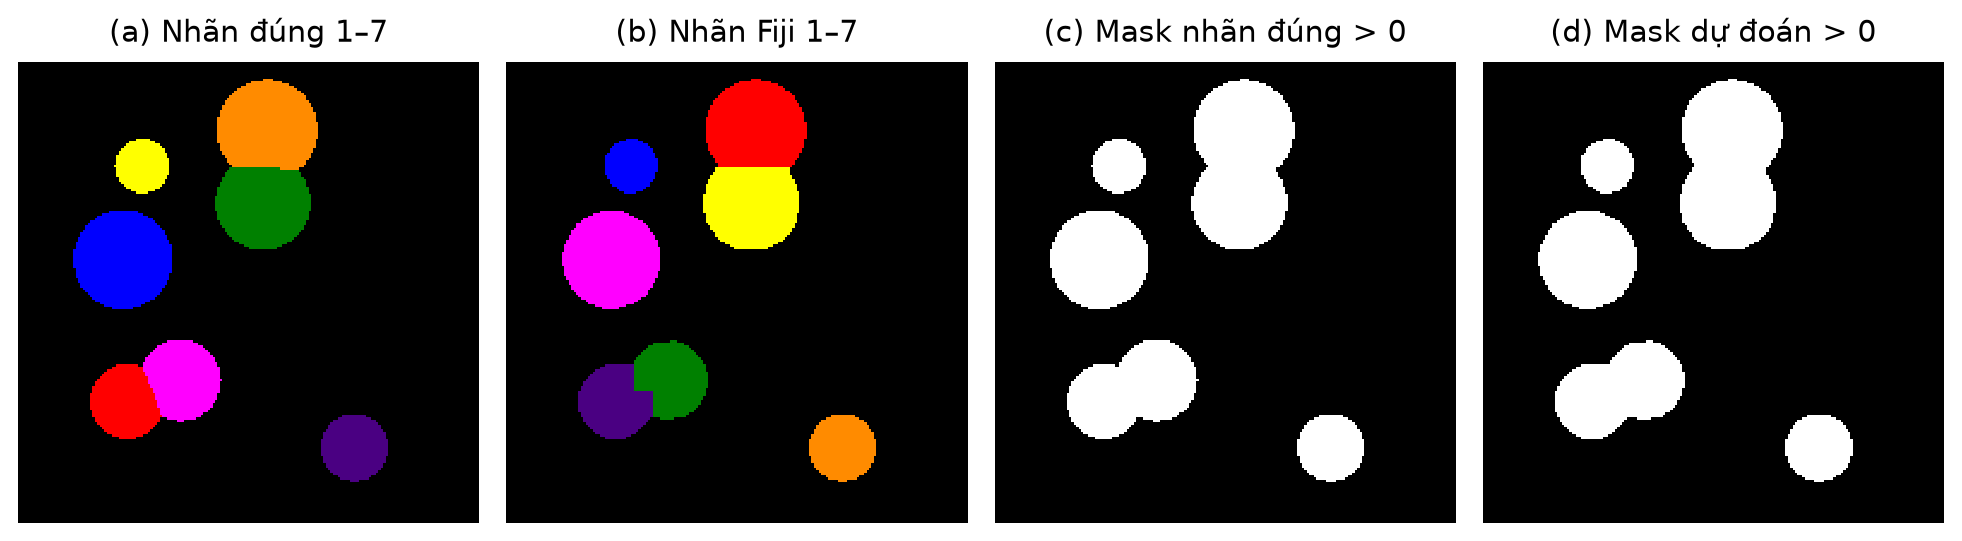
\includegraphics[width=\linewidth]{figures/manual_evaluation.png}
\caption{Nhãn đúng, nhãn Fiji và hai mask tiền cảnh được dùng đo. Nhị phân hóa làm mất ID từng vật nên chỉ dùng hai mask cuối để chấm tiền cảnh.}\label{fig:manual-evaluation}
\end{figure}

\begin{table}[htbp]\centering\small
\caption{Chấm kết quả Fiji làm tay: GUI và code độc lập khớp trong sai số hiển thị.}\label{tab:manual-metrics}
\begin{tabularx}{\linewidth}{X r r}\toprule
Chỉ số & Fiji GUI & Python chấm TIFF Fiji\\\midrule
IoU/Jaccard tiền cảnh & 0,980451 & 0,98045089\\
Dice tiền cảnh & 0,990129 & 0,99012896\\
Số nhãn dự đoán & 7 & 7\\
F1 đối tượng tại IoU $\geq 0,5$ & Không đo ở bảng này & 1,000000\\
TP / FP / FN & Không đo ở bảng này & 7 / 0 / 0\\\bottomrule
\end{tabularx}\end{table}
F1=1 chỉ có nghĩa đủ bảy cặp ghép hợp lệ, không phải mọi pixel đúng. Biên còn khác nhãn đúng nên IoU thấp hơn 1. Kết quả thao tác tay được tách khỏi baseline native tự động (IoU khoảng 0,980132) và Python mặc định (khoảng 0,981397). Một ảnh đơn giản minh họa quy trình; đánh giá nhiều ảnh nằm ở Chương~\ref{chap:experiments}.

\section{Tự động hóa sau khi hiểu thao tác}
Groovy là ngôn ngữ chạy trên Java, có thể gọi API ImageJ/MorphoLibJ trong Fiji Script Editor. \textbf{File $\to$ New $\to$ Script}, mở \path{fiji/Full_Pipeline_Tutorial.groovy}, chọn Language=Groovy rồi Run để chạy từ ảnh gốc theo giao thức cố định. \path{fiji/ReplayWatershed.groovy} chỉ chạy lại bước Watershed từ ba TIFF. Recorder tại \textbf{Plugins $\to$ Macros $\to$ Record} giúp ghi các lệnh menu có hỗ trợ. Chạy lại trên bản sao để kiểm tra script, không giả định Recorder ghi được mọi thao tác.

Trong đánh giá tự động, Fiji shared nhận cùng elevation/markers/mask với Python để kiểm chứng bước Watershed. Fiji native tự xử lý từ ảnh xám chuẩn hóa, dùng 8-bit, SE vuông và ImageJ EDM. Python mặc định dùng float, SE đĩa và EDT tự cài. Khác biệt cả pipeline không được quy về riêng hàm Watershed. Thời gian native có ghi TIFF, không so trực tiếp với thời gian kernel shared để công bố tốc độ.

\chapter{Cài đặt và tổ chức quy trình Python}\label{chap:implementation}

\section{Quy trình Python hoàn chỉnh}
Ảnh được đọc, kiểm tra kích thước và chuẩn hóa. Gaussian sigma=1 làm trơn trước Otsu mặc định. Tiền cảnh sáng sử dụng điều kiện I>T; nếu đối tượng tối dùng I<T. Ngưỡng -1 trong cấu hình yêu cầu Otsu, còn [0,1] là ngưỡng thủ công.

Tiếp theo là hình thái theo operation, lấp lỗ nếu bật và loại thành phần có diện tích nhỏ hơn min\_area. Gán lại nhãn thành phần, tính khoảng cách, tạo marker theo mode và chạy Watershed trên âm khoảng cách. Sau cùng gán lại ID liên tiếp và xuất các giai đoạn để kiểm tra.

\begin{table}[H]\centering\small
\caption{Cấu hình Python mặc định dùng trong đối chiếu chính.}\label{tab:parameters}
\begin{tabularx}{\linewidth}{X X}
\toprule
\textbf{Tham số} & \textbf{Giá trị} \\ \midrule
engine & custom \\
mode & hmax \\
sigma & 1.0 \\
threshold & -1.0 \\
bright\_foreground & True \\
operation & opening\_reconstruction \\
shape & disk \\
radius & 1 \\
min\_area & 25 \\
fill\_holes & True \\
connectivity & 4 \\
h & 2.0 \\
adaptive\_fraction & 0.15 \\
\bottomrule\end{tabularx}\end{table}


Hai engine dùng cùng cấu hình nhưng có triển khai riêng: custom là các hàm tự viết, library dùng SciPy và scikit-image. Gaussian, Otsu, chuyển ảnh xám, đọc ghi, thống kê vùng và chuẩn hóa không được tuyên bố là tự cài. Việc nêu rõ ranh giới này giúp đánh giá đúng đóng góp lập trình của nhóm.

Thời gian total trong pipeline đo phần xử lý, loại đọc ghi và tính metric bên ngoài. Một số ảnh trung gian như erosion và dilation vẫn được tính để phục vụ nghiên cứu dù không được dùng bởi một mode cụ thể; khi so tốc độ phải giữ cùng phạm vi công việc. Không dùng số này như tốc độ tối thiểu của một chương trình production đã loại bỏ mọi bước minh họa.

\begin{figure}[H]\centering
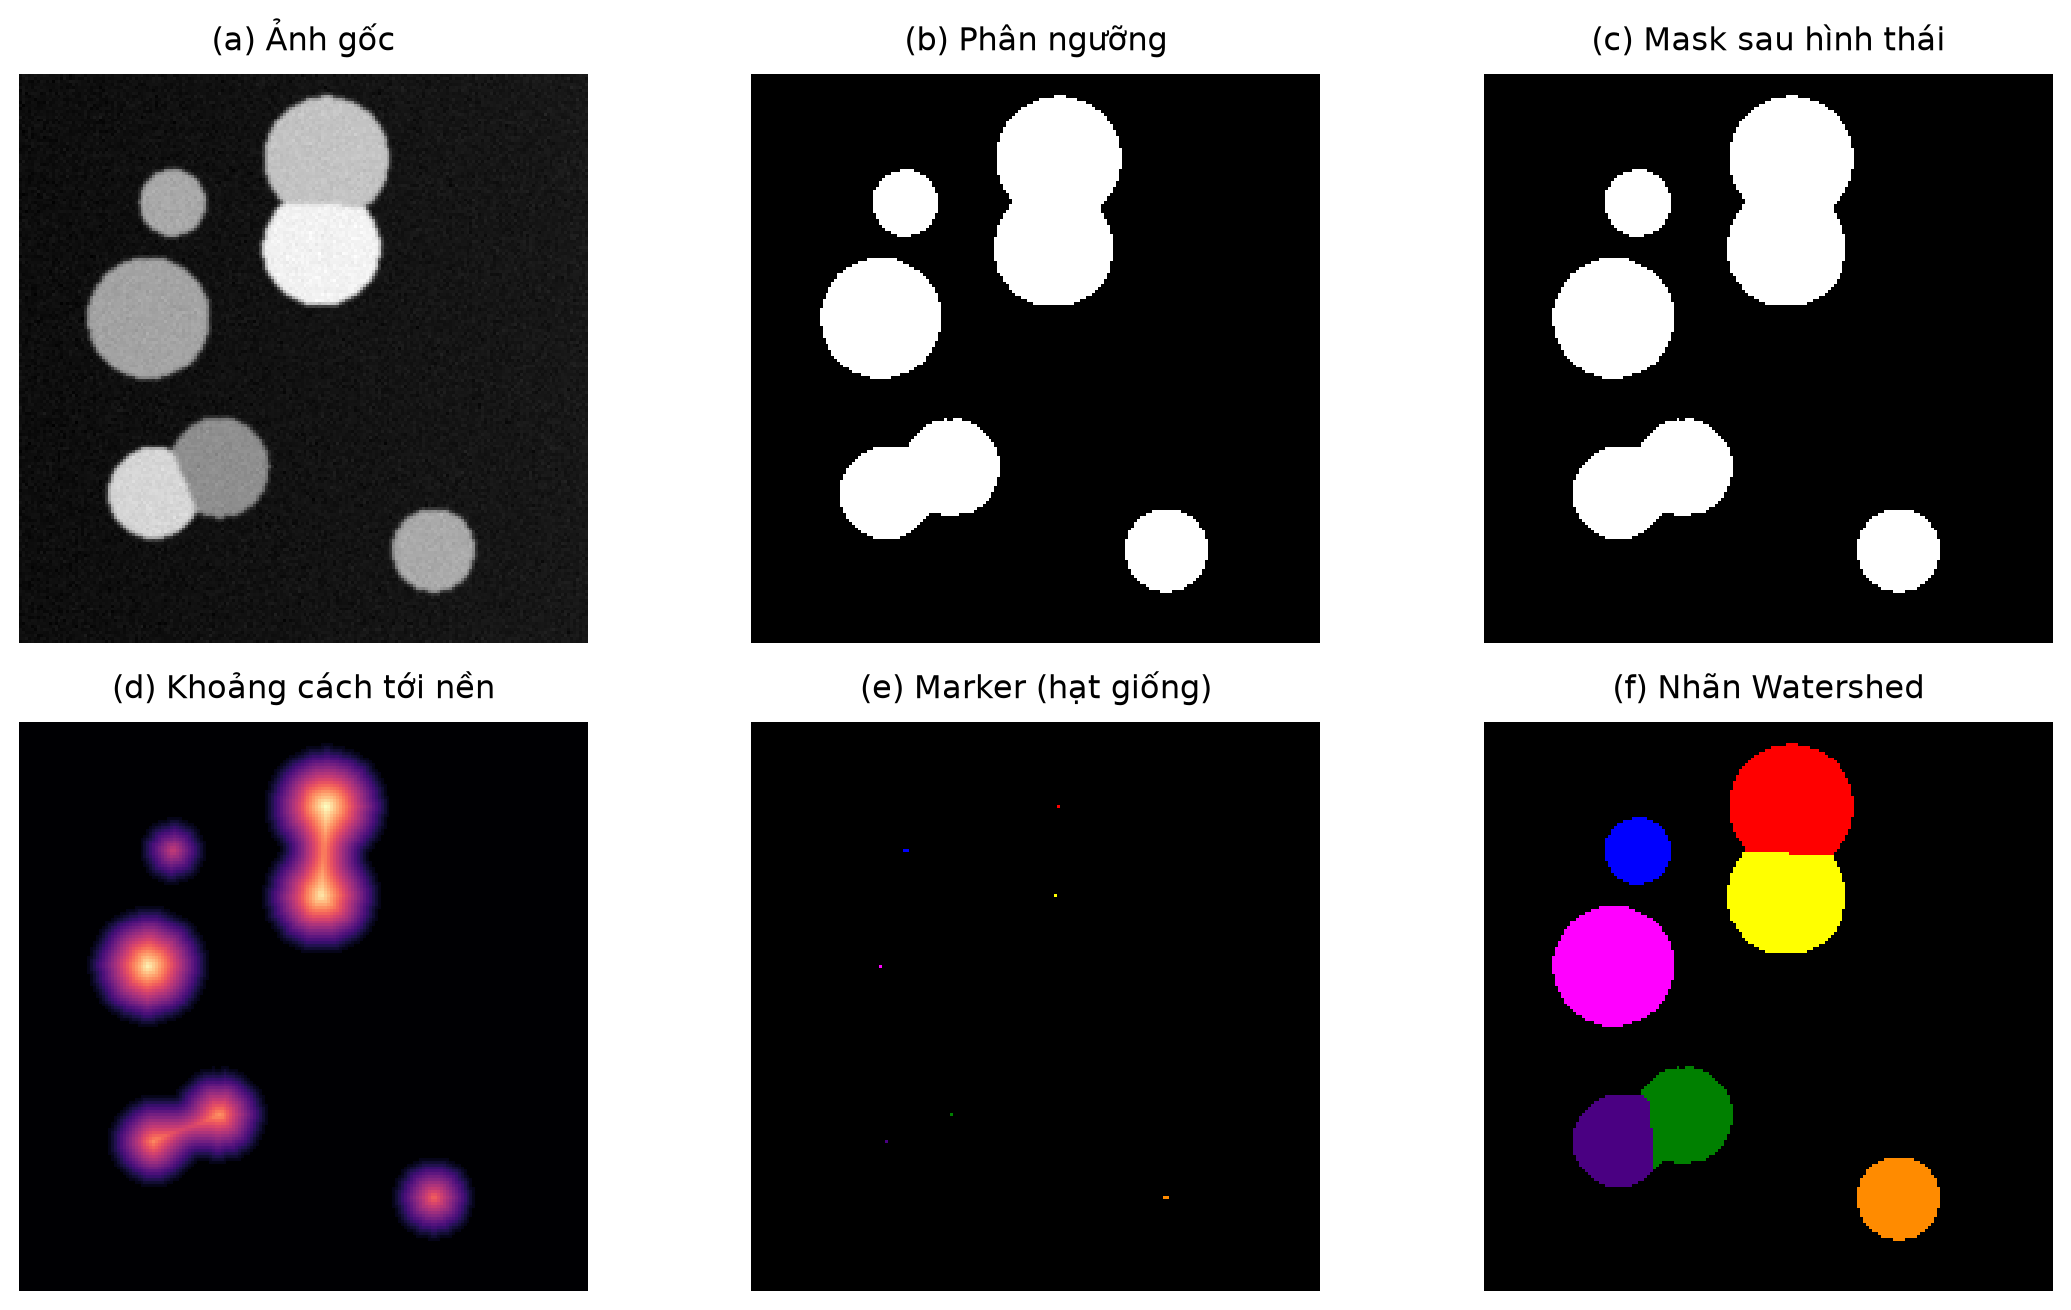
\includegraphics[width=\linewidth]{figures/pipeline.png}
\caption{Sáu bước trên cùng một ảnh: phân ngưỡng, làm sạch mask, khoảng cách, marker và nhãn.}\label{fig:pipeline}
\end{figure}

\section{Cài đặt reconstruction bằng hàng đợi}
Một cách trực tiếp là giãn toàn ảnh lặp đến hội tụ. Nó dễ hiểu nhưng có thể quét lại nhiều pixel đã ổn định. Bản tự cài dùng deque và cờ pending: khi một pixel tăng giá trị, chỉ cần lan ảnh hưởng tới các láng giềng. Cờ pending tránh đưa trùng một pixel vào hàng đợi khi nó đang chờ xử lý.

Trước vòng lặp, chương trình giãn đồng bộ một lượt để tính kết quả ban đầu, rồi chỉ đưa các vị trí tăng so với seed vào hàng đợi. Các vị trí không đổi đã truyền giá trị gốc cho láng giềng trong lượt đồng bộ này. Khi lấy p khỏi hàng đợi, ứng viên của q là min(X[p], F[q]); nếu lớn hơn X[q], cập nhật q và đưa q vào hàng đợi.

\lstinputlisting[caption={Trích mã tự cài: reconstruction\_dilation},label={lst:reconstruction_dilation}]{code/reconstruction_dilation.py}

Hàm kiểm tra cùng kích thước, dữ liệu hữu hạn và seed\ensuremath{\leq}mask. Các phép thử ảnh xám ngẫu nhiên đối chiếu với scikit-image trên liên thông 4 và 8. Tính đúng được xác nhận bằng đầu ra, không suy luận chỉ từ việc chương trình chạy xong. Hiệu quả tốc độ còn phụ thuộc số lần cập nhật và chi phí vòng lặp Python; phần thực nghiệm tối ưu trình bày phép đo thực tế.

\section{Tính khoảng cách bằng bao dưới của parabol}
Trong một chiều, mỗi vị trí nền sinh một parabol bình phương khoảng cách. Hai vị trí i và j có điểm giao s bằng công thức bên dưới. Mảng v giữ các chỉ số parabol còn hữu ích; mảng z giữ mốc giao. Khi một parabol mới làm mốc giao lùi trước miền hiệu lực của parabol cuối, loại parabol cuối khỏi bao.

\begin{equation}s=\frac{(f(j)+j^2)-(f(i)+i^2)}{2(j-i)}\end{equation}

\lstinputlisting[caption={Trích mã tự cài: \_squared\_edt\_1d},label={lst:_squared_edt_1d}]{code/_squared_edt_1d.py}

Sau khi có bao, quét x tăng dần để xác định parabol hiệu lực rồi tính giá trị. Hai lượt hàng và cột dùng chung hàm. Kiểm thử so sánh với scipy.ndimage.distance\_transform\_edt trên ảnh ngẫu nhiên, ảnh rỗng và ảnh toàn tiền cảnh với cùng quy ước khung nền.

Với khối vuông 3\ensuremath{\times}3 đặt giữa nền, distance map trong khối là [1,1,1; 1,2,1; 1,1,1]. Cực đại tại tâm có độ cao 2. Kết quả này giải thích trực tiếp vì sao khoảng cách có thể xác định vùng sâu bên trong vật thể, nhưng một vật thể dài hoặc không lồi vẫn có thể sinh nhiều cực đại.

\section{Mã cài đặt Watershed}
Mã dưới đây là phần tự cài trong morpholab/algorithms.py. Nó sử dụng heapq của Python làm cấu trúc dữ liệu hàng đợi, không gọi hàm watershed của thư viện để tạo kết quả custom. Các cấu trúc deque và heapq là tiện ích lập trình, cần phân biệt với việc sử dụng sẵn toàn bộ thuật toán phân đoạn.

\lstinputlisting[caption={Trích mã tự cài: watershed},label={lst:watershed}]{code/watershed.py}

Thí nghiệm cần lưu chính elevation, markers, mask và connectivity mà hàm này nhận. Một ảnh overlay đơn lẻ không đủ để tái lập, vì thay đổi tiền xử lý hoặc marker có thể thay đổi mạnh số vùng và đường biên. Dữ liệu xuất của dự án chứa các TIFF trung gian và run.json để đáp ứng yêu cầu này.

\section{Chấm nhãn Fiji làm tay và so với Python tự cài}
Sau khi lưu kết quả menu Fiji, dùng đúng nhãn gốc để tính F1, không dùng mask đã gom các ID. Bộ minh chứng đã đặt tên ổn định trong repository nên có thể chấm lại mà không cần thư mục thực hành của người học:
\begin{lstlisting}[language={},numbers=none]
python -m morpholab evaluate ^
 docs/evidence/fiji_manual/ground_truth.tif ^
 docs/evidence/fiji_manual/labels.tif ^
 --out outputs/manual_fiji_metrics.json
python -m morpholab segment ^
 docs/evidence/fiji_manual/input_16bit.tif ^
 --truth docs/evidence/fiji_manual/ground_truth.tif ^
 --config configs/default.json --out outputs/python_example
\end{lstlisting}
Python tự cài có 7 đối tượng, F1=1, IoU khoảng 0,981397 và Dice 0,990611. Fiji làm tay cũng 7 đối tượng và F1=1, nhưng IoU/Dice là 0,980451/0,990129. Hai quy trình có tiền xử lý và SE khác nhau nên không đòi từng pixel trùng. Chấm cả hai với cùng ground truth để phân biệt độ đúng và độ đồng thuận.

Muốn cô lập riêng bước Watershed, chạy Fiji shared nhận cùng elevation, marker, mask và liên thông. Kết quả có thể khác ID nhưng vẫn cùng vùng nên bộ so sánh ghép nhãn trước khi tính đồng thuận. Không dùng màu LUT để so kết quả hoặc xem Fiji là nhãn đúng.

\section{Phân biệt dữ liệu chính, ảnh minh họa và file thông số}
Một lệnh segment lưu nhiều tệp để truy vết; không phải 17 lần xử lý thủ công. Chuỗi chính là gray, smoothed, binary, morphology, mask, distance; từ distance tạo elevation và marker; Watershed nhận đồng thời elevation/markers/mask rồi xuất labels. Erosion/dilation còn dùng khảo sát riêng; components là đối chứng trước tách và hỗ trợ seed dự phòng. Labels RGB và overlay chỉ để xem; objects.csv đo từng vùng, metrics.json chấm với nhãn đúng, run.json ghi tham số và thời gian. Không dùng PNG màu thay TIFF ID khi đánh giá.

Các file code chính có chú thích tiếng Việt: algorithms.py cài toán tử; pipeline.py ghép quy trình; metrics.py chấm điểm; studies.py và benchmark.py chạy khảo sát; fiji.py điều phối tham chiếu. gui.py và ui.py chỉ cung cấp giao diện gọi lại cùng phần lõi. Vì vậy nghiên cứu có thể tái lập hoàn toàn bằng lệnh và menu Fiji trước khi dùng phần mở rộng ứng dụng.
\chapter{Thiết kế thực nghiệm, kết quả và đánh giá}\label{chap:experiments}

\section{Dataset và nhãn đúng}
Nghiên cứu sử dụng hai nguồn dữ liệu. Bộ tổng hợp gồm 18 ảnh 192\ensuremath{\times}192 với seed 20261108, chia 6 validation và 12 test. Các đĩa có độ sáng, kích thước và vị trí biến thiên; vùng giao được phân cho tâm có khoảng cách chuẩn hóa nhỏ nhất. Nhãn hình học được tạo đồng thời với ảnh nên kiểm tra được lỗi tách. Đây là mô hình hóa đơn giản, không đại diện đầy đủ ảnh tế bào.

BBBC039v1 là bộ ảnh nhân tế bào U2OS huỳnh quang do Broad Bioimage Benchmark Collection cung cấp \cite{ref4}. Dữ liệu gồm 200 ảnh TIFF 16-bit kích thước 520\ensuremath{\times}696 và annotation PNG. Dự án giữ phân chia chính thức 100 training, 50 validation và 50 test. Các ảnh cùng nguồn thí nghiệm có thể còn tương quan; 200 ảnh không đồng nghĩa với 200 thí nghiệm sinh học độc lập.

Annotation PNG cần giải mã, không dùng trực tiếp màu như số nhãn. Dự án gán nhãn các vùng liên thông có cùng giá trị trên kênh đầu, nền 0, liên thông 8 theo ví dụ của tác giả \cite{ref5}. Manifest lưu tên ảnh, split, đường dẫn ảnh và nhãn, cùng checksum của archive để kiểm tra nguồn.

Chưa huấn luyện mô hình nên training không được dùng để cập nhật trọng số. Validation chọn tham số và khảo sát phương án. Test dùng báo cáo cuối trên cấu hình đã cố định. Nếu phát triển tiếp sau khi xem test, phải công khai rằng tập test này đã tham gia vòng phát triển và cần dữ liệu đánh giá độc lập mới để xác nhận cải tiến.

\begin{figure}[H]\centering
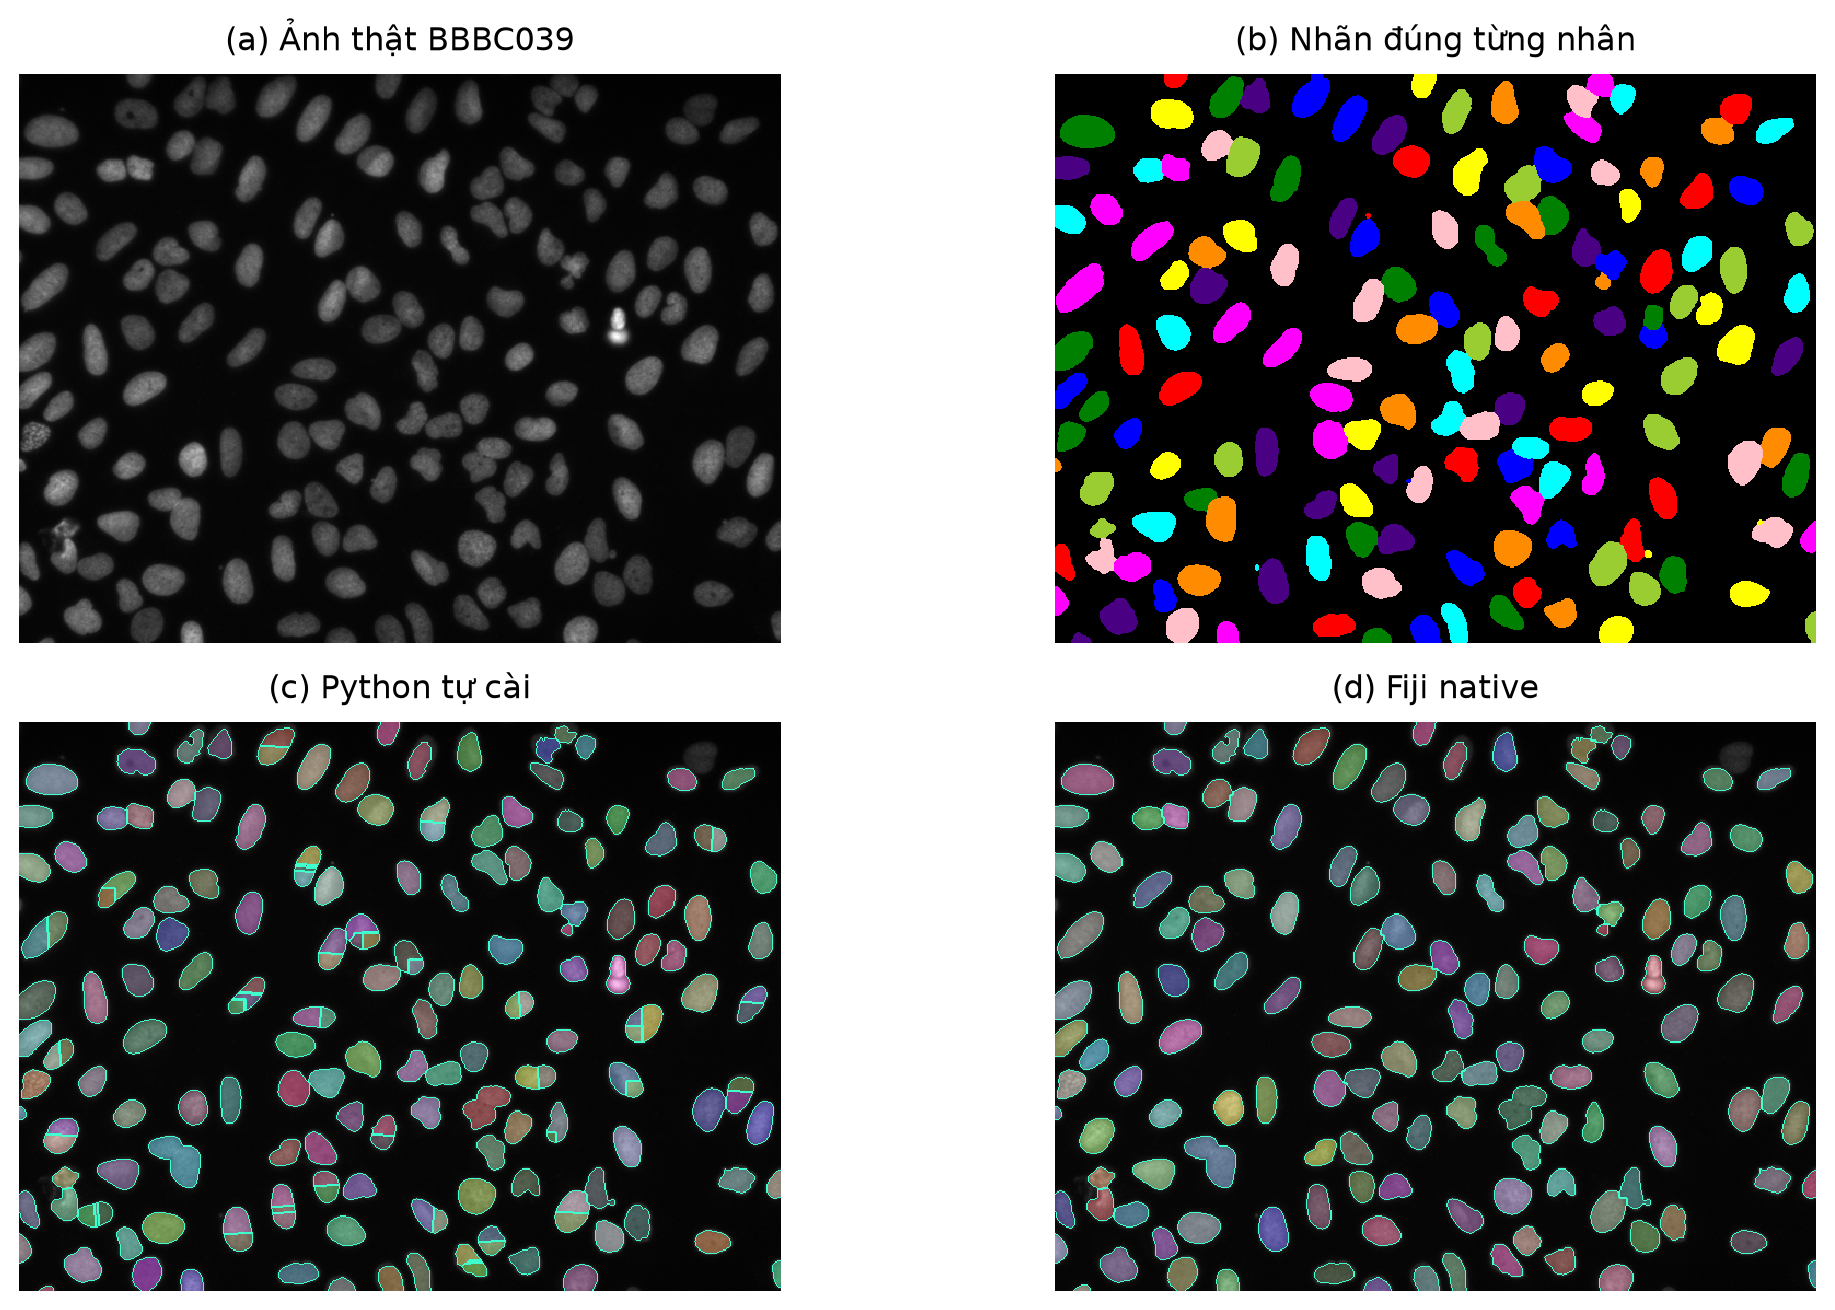
\includegraphics[width=\linewidth]{figures/real_example.png}
\caption{Ví dụ ảnh thật BBBC039, nhãn đúng và kết quả Python/Fiji native. Cùng ảnh test; màu ID chỉ hỗ trợ nhìn vùng.}\label{fig:real}
\end{figure}

\section{Chỉ số định lượng và cách ghép đối tượng}
IoU và Dice tiền cảnh đánh giá mức trùng nhau của hai mặt nạ, không phân biệt các nhãn bên trong. F1 theo đối tượng cần ghép nhãn dự đoán với nhãn đúng. Dự án chỉ cho ghép cặp có IoU\ensuremath{\geq}0,5; mỗi nhãn dùng tối đa một lần. Hungarian tối đa số cặp hợp lệ trước, rồi tối đa tổng IoU trong các cặp đó.

\begin{equation}\mathrm{IoU}=\frac{|P\cap G|}{|P\cup G|},\qquad\mathrm{Dice}=\frac{2|P\cap G|}{|P|+|G|}\end{equation}
\begin{equation}\mathrm{Precision}=\frac{TP}{TP+FP},\quad\mathrm{Recall}=\frac{TP}{TP+FN},\quad F_1=\frac{2TP}{2TP+FP+FN}\end{equation}
\begin{equation}\mathrm{PQ}=\frac{\sum_{\text{cặp đúng}}\mathrm{IoU}}{TP+0.5FP+0.5FN}\end{equation}

TP là số cặp ghép đúng; FP là dự đoán chưa ghép; FN là vật thể thật bị bỏ sót. Sai số đếm tuyệt đối là |n\_pred-n\_true|. Khi cả hai ảnh rỗng, IoU/Dice/F1 quy ước bằng 1; nếu chỉ một ảnh rỗng, F1 bằng 0. Quy ước này được kiểm thử và phải đọc cùng số vật thể, tránh hiểu “ảnh không có gì đạt 100\%” là kết quả phân đoạn tốt trên ảnh có đối tượng.

Split/merge dùng một quan hệ chẩn đoán: hai vùng có giao ít nhất 10\% diện tích vùng nhỏ hơn. Một nhãn thật liên hệ với nhiều dự đoán là split; một dự đoán liên hệ với nhiều nhãn thật là merge. Đây không phải số lỗi tuyệt đối duy nhất theo mọi chuẩn đánh giá, mà là quy ước minh bạch của dự án.

So Fiji với Python sử dụng phép ghép ID riêng theo số pixel giao để đo đồng thuận trên hợp tiền cảnh. Đồng thuận cao chỉ cho thấy hai triển khai gần nhau. Muốn nói đúng với vật thể thật vẫn phải dùng ground truth.

\section{Thiết kế thí nghiệm và kiểm soát sai lệch}
Thí nghiệm so sánh bốn cách chạy trên cùng 50 ảnh test: Python custom, Python library, Fiji shared và Fiji native. Cấu hình Python cố định hmax, sigma=1, Otsu, SE đĩa bán kính 1, min\_area=25, h=2, liên thông 4, đối tượng sáng và lấp lỗ. Fiji native sử dụng quy ước riêng đã nêu. Mỗi hàng per\_image.csv là một cặp ảnh và cách chạy.

Khảo sát h ban đầu chạy library/hmax trên 6 ảnh validation đầu với h\ensuremath{\in}\{0,5;1;2;4;6\}. Kết quả chọn h=2. Từ bản 1.2, chức năng sweep tôn trọng engine đang chọn và xuất đúng mode hmax. Khi tái lập số liệu cũ, dùng cấu hình library; không thay engine rồi cho rằng đó là cùng một thí nghiệm.

Phép ablation gồm baseline, bỏ Gaussian, bỏ hình thái, opening thường, bỏ lấp lỗ, marker raw và CCL. Khảo sát độ bền gồm ảnh gốc, nhiễu Gaussian \ensuremath{\sigma}=0,02/0,05/0,1 và làm mờ \ensuremath{\sigma}=1/2/3. Mỗi khảo sát dùng 6 validation, tổng 42 dòng. Các ảnh biến đổi cùng nguồn không được tính như các mẫu độc lập mới.

Python có một lượt warm-up trước đo. Đợt so sánh đã lưu dùng một lượt đo mỗi cấu hình mỗi ảnh; do đó số thời gian là mô tả, chưa đủ kết luận ổn định. Công cụ cho phép tăng repeats và lấy trung vị. Chất lượng lấy trung bình F1 theo ảnh, không gộp mọi vật thể của cả tập thành một ảnh lớn.

CI 95\% được tính bằng bootstrap percentile 1000 lần lấy mẫu ảnh với seed cố định. CI thể hiện biến thiên trong tập khảo sát; các khoảng chồng lấn hoặc không chồng lấn không tự thay cho kiểm định cặp hay nghiên cứu trên dữ liệu độc lập.

\begin{figure}[H]\centering
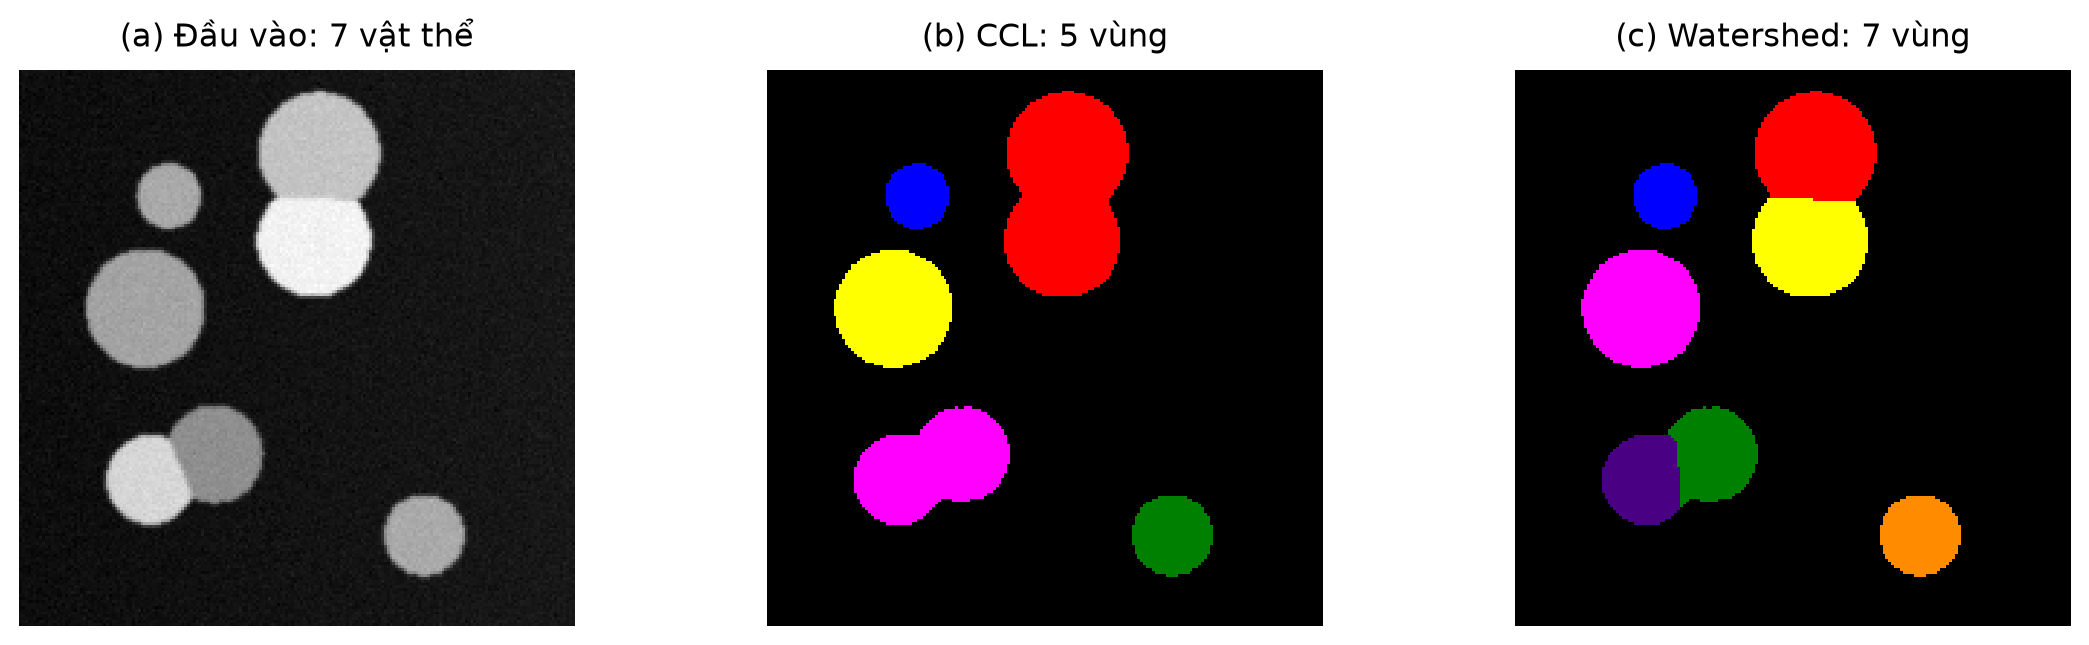
\includegraphics[width=\linewidth]{figures/ccl_watershed.png}
\caption{Ví dụ có 7 vật thể: CCL trả 5 vùng, Watershed có marker trả 7. Không suy rộng từ một ảnh mẫu.}\label{fig:ccl}
\end{figure}

\section{Kết quả đối chiếu trên 50 ảnh test}
\begin{table}[H]\centering\small
\caption{Đối chiếu trên 50 ảnh test BBBC039; trung bình theo ảnh.}\label{tab:compare}
\begin{tabularx}{\linewidth}{p{0.21\linewidth} p{0.05\linewidth} X p{0.22\linewidth} X X}
\toprule
\textbf{Cách chạy} & \textbf{Ảnh} & \textbf{F1} & \textbf{CI 95\%} & \textbf{IoU} & \textbf{MAE đếm} \\ \midrule
python-custom & 50 & 0.7087 & 0.6807–0.7305 & 0.8954 & 21.10 \\
python-library & 50 & 0.7054 & 0.6771–0.7277 & 0.8954 & 21.10 \\
fiji-shared & 50 & 0.7188 & 0.6914–0.7386 & 0.8954 & 21.10 \\
fiji-native & 50 & 0.8917 & 0.8592–0.9132 & 0.8910 & 13.58 \\
\bottomrule\end{tabularx}\end{table}



\begin{figure}[H]\centering
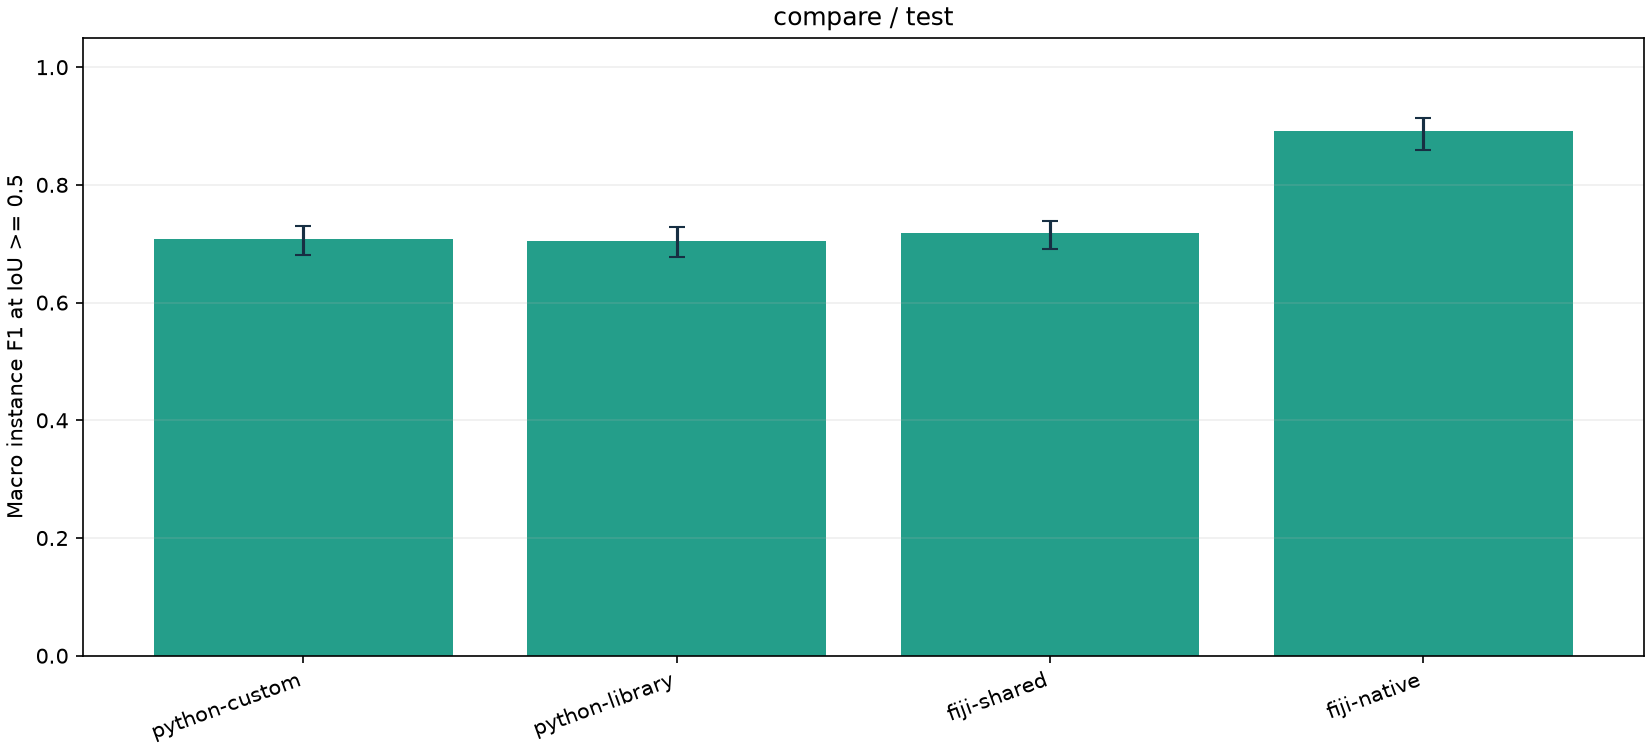
\includegraphics[width=\linewidth]{figures/v2_compare_bbbc039_test.png}
\caption{F1 trung bình và khoảng tin cậy bootstrap 95\% trên 50 ảnh test.}\label{fig:compare}
\end{figure}


Python custom, Python library và Fiji shared có cùng IoU tiền cảnh khoảng 0,8954 và sai số đếm trung bình 21,10, nhưng F1 khác nhau. Điều này phù hợp với việc chúng chia cùng mask thành cùng số nhãn nhưng đường biên giữa các nhãn không hoàn toàn giống nhau. Trung vị đồng thuận pixel của shared so với custom khoảng 95,56\%.

Fiji native đạt F1 0,8917 trên tập này, đồng thời IoU tiền cảnh 0,8910 thấp hơn nhẹ. Kết quả cho thấy chất lượng mask và chất lượng tách đối tượng là hai tiêu chí khác nhau. Native có ít split hơn rõ rệt nhưng vẫn có merge; không có cơ sở kết luận mọi ảnh hoặc mọi miền dữ liệu đều tốt hơn.

Dữ liệu nguồn gồm 200 dòng không lỗi. CSV và study.json được lưu tại docs/evidence/v2\_compare\_bbbc039\_test. Biểu đồ và bảng trong báo cáo được lấy từ dữ liệu đã đo, không lấy số từ ảnh chụp GUI hay kết quả công bố của phương pháp khác.

\section{Phân tích ảnh hưởng của từng bước}
\begin{table}[H]\centering\small
\caption{Loại/thay từng bước trên 6 ảnh validation.}\label{tab:ablation}
\begin{tabularx}{\linewidth}{p{0.35\linewidth} X X X}
\toprule
\textbf{Biến thể} & \textbf{F1} & \textbf{IoU} & \textbf{MAE đếm} \\ \midrule
baseline & 0.6663 & 0.8798 & 24.5000 \\
no gaussian & 0.6884 & 0.8904 & 22.3333 \\
no morphology & 0.6663 & 0.8798 & 24.5000 \\
ordinary opening & 0.6692 & 0.8787 & 24.3333 \\
no fill holes & 0.6592 & 0.8791 & 25.3333 \\
raw markers & 0.1563 & 0.8798 & 298.5000 \\
connected components & 0.8168 & 0.8798 & 16.3333 \\
\bottomrule\end{tabularx}\end{table}



\begin{figure}[H]\centering
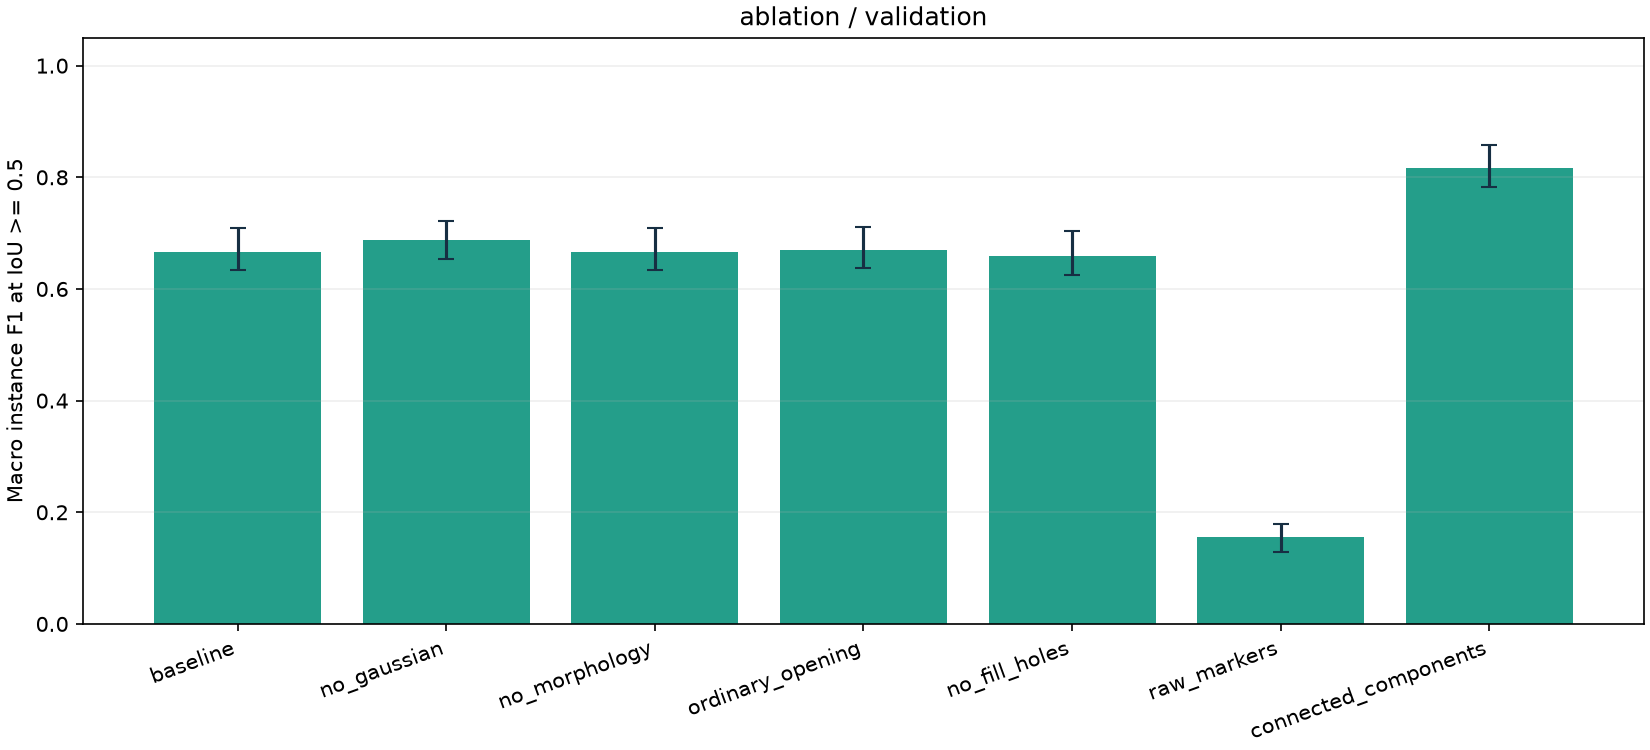
\includegraphics[width=\linewidth]{figures/v2_ablation_bbbc039.png}
\caption{Ablation: ảnh hưởng của từng bước trên 6 ảnh validation.}\label{fig:ablation}
\end{figure}


Trên sáu ảnh validation này, bỏ Gaussian tăng F1 từ 0,6663 lên 0,6884; bỏ hình thái không thay đổi F1 ở cấu hình hiện tại. Marker raw làm F1 giảm mạnh còn 0,1563 và tạo nhiều split. CCL đạt 0,8168, cao hơn baseline Watershed, cho thấy marker ở baseline vẫn có xu hướng chia thừa trên các ảnh khảo sát.

Các kết quả không có nghĩa Gaussian hoặc reconstruction luôn vô ích. Tác dụng phụ thuộc độ nhiễu, kích thước SE, cấu trúc vật thể và cách chọn marker. Phép thử chỉ thay một yếu tố trong cấu hình hiện tại, chưa khảo sát tương tác giữa nhiều tham số. Việc giữ một bước trong quy trình cần được giải thích bằng giả thuyết và số liệu, không dựa vào số lượng bước càng nhiều càng tốt.

Một hướng phát triển hợp lý là chọn marker ổn định hơn và khảo sát h cùng sigma trên validation. Đề xuất này chưa được chứng minh là tăng điểm trên dữ liệu độc lập; báo cáo không nâng nó thành kết luận thực nghiệm.

\section{Ảnh hưởng của nhiễu và làm mờ}
\begin{table}[H]\centering\small
\caption{Nhiễu và làm mờ trên 6 ảnh validation.}\label{tab:robustness}
\begin{tabularx}{\linewidth}{p{0.35\linewidth} X X X}
\toprule
\textbf{Biến thể} & \textbf{F1} & \textbf{IoU} & \textbf{MAE đếm} \\ \midrule
clean & 0.6663 & 0.8798 & 24.5000 \\
noise 0.02 & 0.6527 & 0.8736 & 23.6667 \\
noise 0.05 & 0.6668 & 0.8374 & 18.8333 \\
noise 0.1 & 0.6385 & 0.7792 & 18.0000 \\
blur 1 & 0.6689 & 0.8751 & 21.6667 \\
blur 2 & 0.6406 & 0.8616 & 19.3333 \\
blur 3 & 0.6018 & 0.8461 & 20.3333 \\
\bottomrule\end{tabularx}\end{table}



\begin{figure}[H]\centering
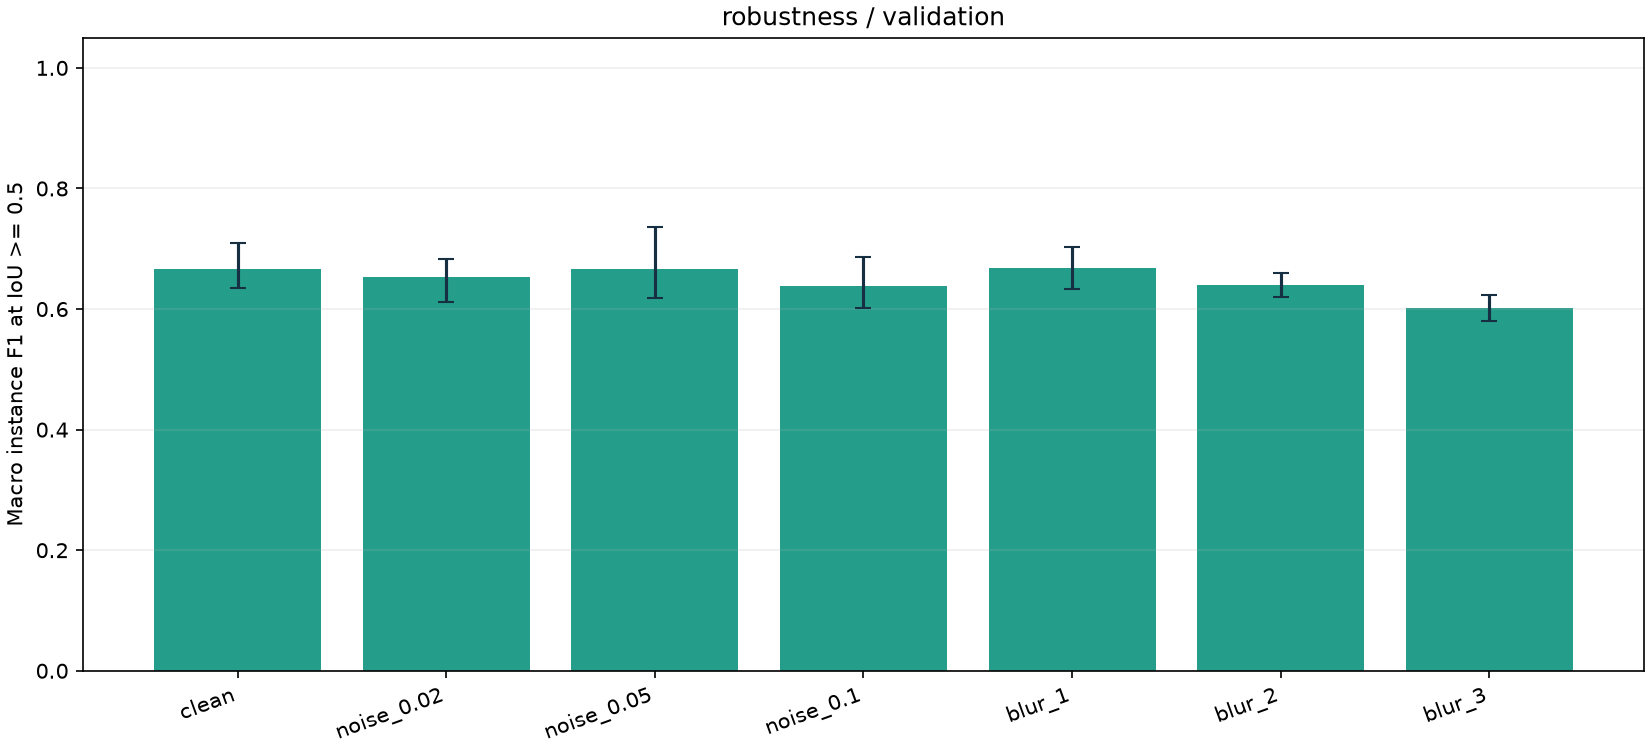
\includegraphics[width=\linewidth]{figures/v2_robustness_bbbc039.png}
\caption{Robustness: biến đổi nhiễu/làm mờ trên cùng 6 ảnh validation.}\label{fig:robustness}
\end{figure}


F1 của ảnh gốc khoảng 0,6663; khi làm mờ sigma=3 giảm còn 0,6018. IoU tiền cảnh cũng giảm, cho thấy mất chi tiết biên ảnh hưởng đến cả mask và marker. Nhiễu nhẹ không tạo xu hướng đơn điệu tuyệt đối của F1 trên tập nhỏ, vì một thay đổi cường độ có thể làm số marker tăng hoặc giảm theo những cách khác nhau.

Nhiễu được thêm sau chuẩn hóa và clip về [0,1]. Làm mờ giữ nguyên nhãn đúng để đo sức chịu đựng của thuật toán trước suy giảm ảnh; không tạo nhãn mới thích ứng với ảnh đã mờ. Đây là stress test có kiểm soát, không phải mô phỏng đầy đủ mọi nguồn nhiễu của kính hiển vi.

Kết quả cần đọc cùng ảnh trung gian. Nếu mask đã mất một vùng, Watershed không thể tạo lại vùng đó từ nền bị loại. Nếu mask vẫn tốt nhưng marker quá dày, lỗi chủ yếu nằm ở bước chia đối tượng. Việc lưu từng giai đoạn giúp phân biệt hai nguyên nhân này và đề xuất sửa đúng chỗ.

\section{Benchmark và thực nghiệm tối ưu}
\begin{table}[H]\centering\small
\caption{Thời gian reconstruction: 5 lần đo sau 1 warm-up, đầu ra bằng nhau.}\label{tab:timing}
\begin{tabularx}{\linewidth}{p{0.10\linewidth} p{0.30\linewidth} X X X}
\toprule
\textbf{Cạnh ảnh} & \textbf{Cách cài} & \textbf{Trung vị (s)} & \textbf{Min (s)} & \textbf{Max (s)} \\ \midrule
48 & queue python & 0.008983 & 0.008805 & 0.009617 \\
48 & synchronous scipy & 0.002225 & 0.002203 & 0.002262 \\
96 & queue python & 0.035766 & 0.035478 & 0.036634 \\
96 & synchronous scipy & 0.009409 & 0.008918 & 0.011008 \\
160 & queue python & 0.100107 & 0.098277 & 0.108437 \\
160 & synchronous scipy & 0.030336 & 0.028342 & 0.031392 \\
\bottomrule\end{tabularx}\end{table}


Thí nghiệm bổ sung tạo mask hằng 1 kích thước 48, 96 và 160, với một seed sáng tại tâm, liên thông 4. So sánh reconstruction giãn đồng bộ dùng SciPy với bản hàng đợi Python. Mỗi trường hợp warm-up một lần, đo năm lần, kiểm tra đầu ra giống hệt và loại thời gian đọc ghi khỏi phép đo. Kết quả đầy đủ nằm trong timing.csv và protocol.json.

Bản queue Python chậm hơn bản synchronous dùng SciPy trên cả ba kích thước được thử. Đây là kết quả thực, không phải lỗi cần che đi: số phép cập nhật lý thuyết ít hơn chưa bảo đảm thời gian nhỏ hơn khi một bên dùng vòng lặp Python và một bên gọi nhân xử lý đã biên dịch. Thử nghiệm này so hai triển khai thực tế, không cô lập riêng độ phức tạp thuật toán.

Trong so sánh 50 ảnh, trung vị thời gian pipeline custom khoảng 6,9673 giây và library khoảng 0,3184 giây. Hai bản có cùng mục tiêu đầu ra nhưng chi phí vòng lặp khác. Native gồm ghi ảnh trung gian, shared chỉ đo một bước, nên không đặt tất cả vào cùng phép chia tốc độ. Không dùng đợt đo này để kết luận phần cứng khác sẽ có cùng thời gian.

Cải tiến đã cài gồm dùng lát NumPy cho hình thái, deque có cờ pending cho reconstruction và EDT tách trục tuyến tính. Mỗi cải tiến cần giữ đầu ra đúng qua kiểm thử. Hướng tối ưu tiếp theo là biên dịch vòng lặp nóng hoặc giảm xuất trung gian trong chế độ chạy nhanh, đồng thời đo lại có kiểm soát.

\section{Kiểm thử tính đúng và khả năng tái lập}
Bộ kiểm thử có 29 trường hợp chạy qua trên môi trường đã ghi, gồm thuật toán, metric, Java/Fiji, phiên làm việc và bảy luồng giao diện thực. Các test không chỉ so ảnh bằng mắt: morphology đối chiếu SciPy cả SE bất đối xứng; reconstruction so ảnh xám ngẫu nhiên; EDT kiểm tra biên; CCL thử liên thông; Watershed kiểm tra mask và marker; metric thử hoán vị ID, ảnh rỗng, lỗi split và merge.

FijiIntegrationTest gọi plugin thật và đối chiếu chỉ số Java với Python. Kiểm thử phiên lưu xác nhận ảnh, cấu hình và nhãn được khôi phục. Kiểm thử hủy xác nhận worker dừng và tiến trình con được thu hồi. Biên bản chi tiết nằm trong docs/KIEM\_THU\_PHAN\_MEM.md; số test qua không đồng nghĩa mọi ảnh sẽ phân đoạn đúng.



\par\medskip\noindent\begin{minipage}[t]{\linewidth}
\begin{lstlisting}[language={},numbers=none]
conda activate ai
cd /d D:\XU_LY_ANH
python -B -m unittest discover -s tests -v
python scripts/academic_smoke.py
\end{lstlisting}\end{minipage}\par\medskip



Một phép thử quan trọng cho người dùng là đặt min\_area=100000 trên ảnh 192\ensuremath{\times}192. Toàn ảnh chỉ có 36864 pixel nên mask sau lọc phải rỗng. Với ground truth có vật thể, F1 phải bằng 0; nếu không có ground truth, F1 phải để trống thay vì tự gán một điểm. Đây là kiểm thử hành vi và cách diễn giải, không phải một cấu hình hợp lý để phân đoạn.

Để tái lập, giữ manifest, file cấu hình, phiên bản thư viện, loại dữ liệu và phạm vi tính thời gian. Lệnh có cùng seed tạo cùng ảnh tổng hợp; số thời gian vẫn biến thiên do hệ điều hành và tải máy. Mỗi lần nghiên cứu tạo một thư mục mới để tránh trộn số liệu cũ và mới.
\chapter{Ứng dụng hỗ trợ, tái lập và kết luận}\label{chap:app}
\section{MorphoLab: công cụ hỗ trợ thực nghiệm}
Ứng dụng desktop được xây dựng để giảm thao tác khi đổi tham số, xem ảnh trung gian và chạy kiểm chứng. Phần lõi vẫn là các hàm Python đã trình bày; kết quả gọi từ giao diện và CLI có cùng quy ước dữ liệu. Ứng dụng là sản phẩm bổ trợ cho nghiên cứu, không phải tiêu chí thay thế nội dung thuật toán, thực nghiệm hoặc đánh giá định lượng.

Sáu tab gồm Phân đoạn, Fiji \& đánh giá, Benchmark, Nghiên cứu, Phiên đã lưu và Hướng dẫn. Giao diện giải thích thuật ngữ tiếng Anh bằng tiếng Việt: marker (hạt giống), mask (miền tiền cảnh), ground truth (nhãn đúng), split/merge (chia thừa/gộp sai). Cảnh báo kết quả cũ giúp tránh thay tham số rồi vô tình xuất kết quả của lần chạy trước.

\begin{figure}[htbp]\centering
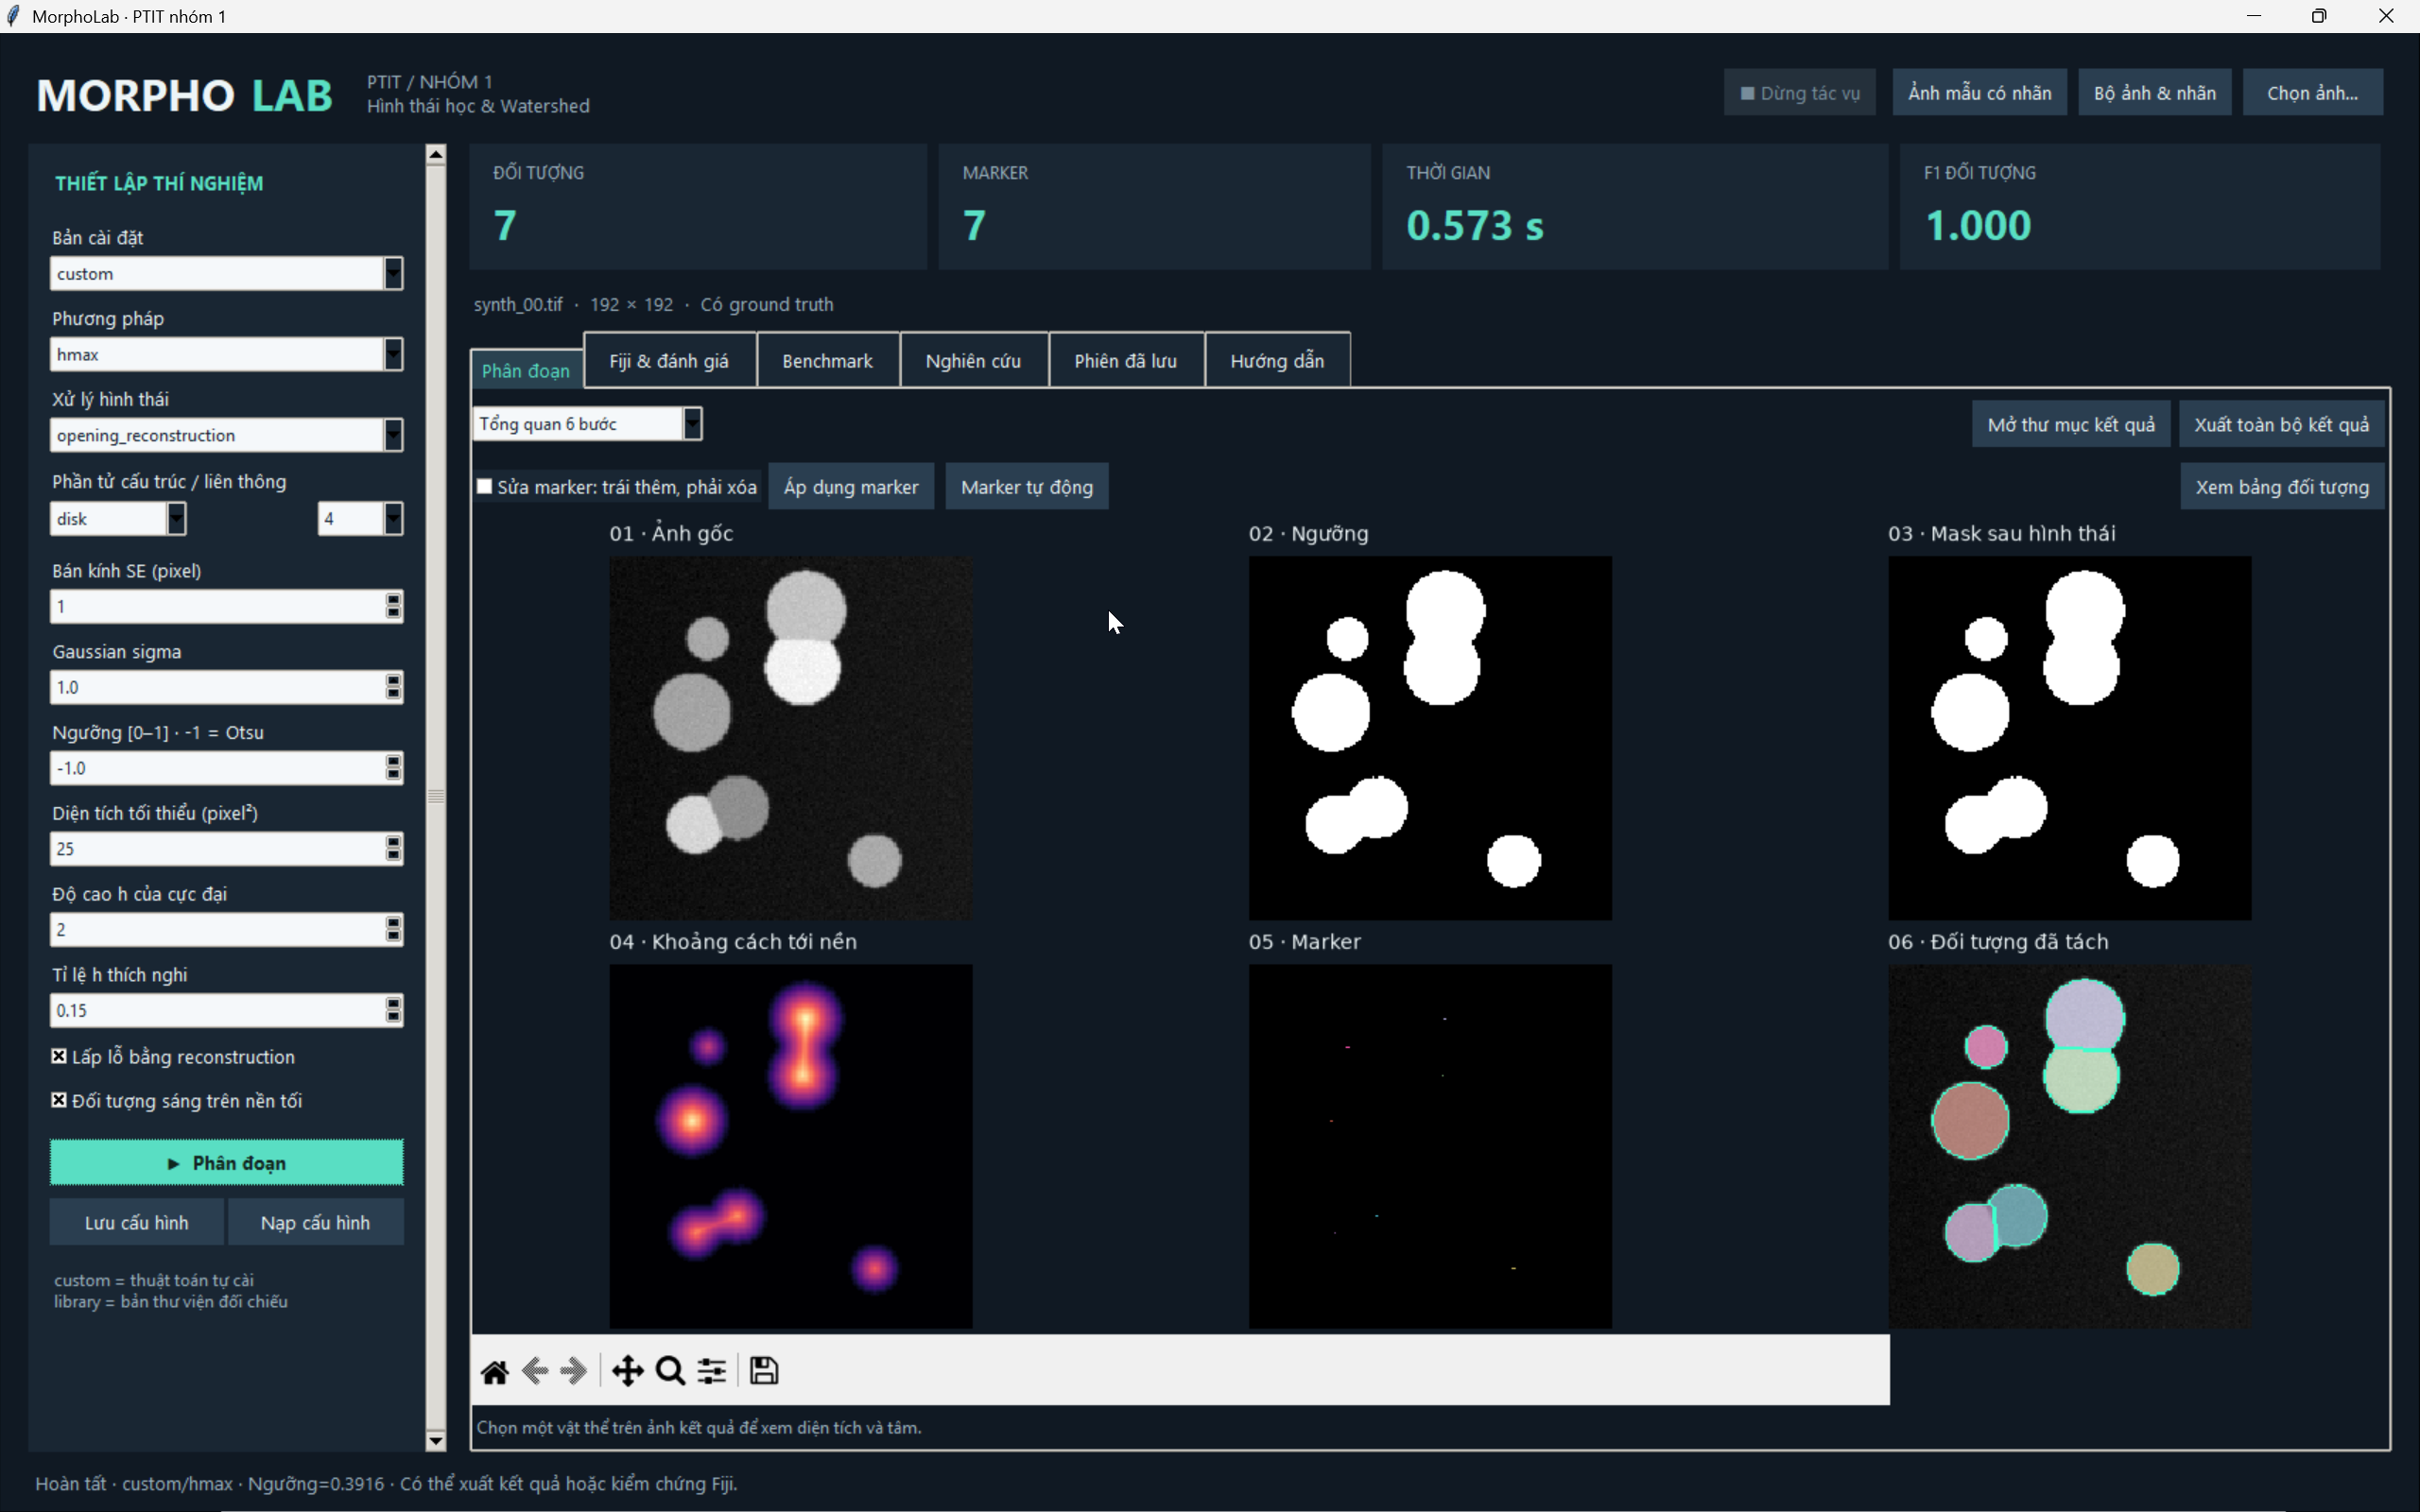
\includegraphics[width=\linewidth]{figures/morpholab_app.png}
\caption{MorphoLab hiển thị sáu bước trên ảnh mẫu: 7 đối tượng, 7 marker, F1 = 1. Ảnh chụp ứng dụng do người học cung cấp trong quá trình thực hành; thời gian hiển thị thuộc lần chạy đó.}\label{fig:app}
\end{figure}

\begin{table}[htbp]\centering\small
\caption{Chức năng ứng dụng gắn với công việc nghiên cứu.}\label{tab:app}
\begin{tabularx}{\linewidth}{X X}\toprule
Chức năng & Giá trị hỗ trợ \\\midrule
Xem sáu bước và từng ảnh trung gian & Giải thích nguyên nhân lỗi từ ngưỡng, mask hoặc marker.\\
Chỉnh marker bằng chuột & Thử giả thuyết về số hạt giống; kết quả thủ công được phân biệt với tự động.\\
Gọi Fiji shared/native & Kiểm chứng JAR thật và xem khác biệt; giữ hai giao thức rõ ràng.\\
Benchmark và kế hoạch nghiên cứu & Chạy nhiều ảnh tuần tự, xuất CSV/JSON/biểu đồ.\\
Lưu/mở phiên & Giữ ảnh, nhãn đúng, cấu hình và đầu ra để xem lại.\\
Xuất bảng đối tượng & Đọc diện tích, tâm và thuộc tính từng nhãn.\\\bottomrule
\end{tabularx}\end{table}

\section{Kịch bản dùng app để minh họa}
Mở \texttt{launch\_app.cmd} hoặc chạy \texttt{python -m morpholab gui} trong env \texttt{ai}. Chọn \textbf{Ảnh mẫu có nhãn}, giữ cấu hình mặc định và bấm \textbf{Phân đoạn ảnh}. Xem lần lượt ảnh gốc, phân ngưỡng, mask, distance, marker và nhãn. Đổi mode sang CCL để thấy năm vùng, rồi trở lại hmax để thấy bảy đối tượng. Mọi thay đổi phải bấm chạy lại trước khi so sánh hoặc xuất.

Sang \textbf{Fiji \& đánh giá}, chạy tham chiếu, xem nhãn Python/Fiji và vùng bất đồng. Nếu sửa marker, cần áp dụng marker trước; không trộn kết quả tương tác với kết quả tự động khi báo cáo F1. Các tab Benchmark/Nghiên cứu dùng cấu hình và dataset đã chọn; bắt đầu một ảnh trước khi chạy cả tập.

\section{Giới hạn của công cụ hỗ trợ}
Giao diện không làm thuật toán tự hiểu ngữ nghĩa ảnh. Thao tác người dùng có thể thay kết quả mạnh nên cấu hình, nhãn đầu vào và lịch sử chạy phải được giữ. Test phần mềm kiểm tra luồng thao tác và xuất dữ liệu, còn chất lượng phân đoạn vẫn phải đo với ground truth. Trong buổi bảo vệ, có thể demo bằng app nhưng phải chỉ được hàm xử lý và lệnh CLI tương ứng để tái lập độc lập.

\section{Hướng dẫn chạy phần nghiên cứu bằng lệnh}
Mở Anaconda Prompt, kích hoạt env ai, chuyển tới thư mục dự án. Không cần mở GUI MorphoLab để thực hiện các bước nghiên cứu. Cần Java JDK trong Fiji vì adapter được biên dịch trước khi chạy. Kiểm tra plugin có tại C:/Tools/Fiji/plugins/MorphoLibJ\_-1.6.5.jar.



\par\medskip\noindent\begin{minipage}[t]{\linewidth}
\begin{lstlisting}[language={},numbers=none]
conda activate ai
cd /d D:\XU_LY_ANH
python -m morpholab dataset synthetic
python -m morpholab segment data\synthetic\synth_00.tif ^
 --truth data\synthetic\synth_00_gt.tif ^
 --out outputs\demo_shared --fiji
python scripts/academic_smoke.py
\end{lstlisting}\end{minipage}\par\medskip



Lệnh segment xuất các TIFF giai đoạn, labels.tif, ảnh màu, bảng đối tượng và run.json. Khi có --truth, thêm metrics.json. Khi có --fiji, thư mục fiji chứa kết quả MorphoLibJ, chỉ số Java, dữ liệu đối chiếu và script Groovy. Chạy --fiji-native vào thư mục khác để giữ hai loại thí nghiệm riêng.

Kết quả mẫu mong đợi với cấu hình mặc định là bảy vật thể và F1 đối tượng bằng 1,000. IoU tiền cảnh không nhất thiết bằng 1 vì ngưỡng và làm trơn có thể làm biên khác nhãn hình học. Thời gian phụ thuộc máy, không dùng một con số thời gian cố định làm điều kiện pass.

Nếu lệnh báo không tìm thấy dữ liệu, chạy dataset synthetic hoặc dataset bbbc039. Nếu lỗi thiếu plugin, kiểm tra IJPB-plugins trong Fiji rồi cập nhật và mở lại. Nếu Java không biên dịch được, kiểm tra đường dẫn Fiji có thư mục java và javac; chi tiết xử lý lỗi và đường dẫn đầu ra có trong hướng dẫn chạy đi kèm.

\section{Kịch bản demo và kiểm tra trực tiếp}
Demo nên đi từ trường hợp hiểu được bằng mắt đến số liệu nhiều ảnh. Đầu tiên trình bày ảnh bảy đĩa, chỉ ra hai cặp chạm nhau. Chạy CCL để quan sát năm vùng, sau đó chạy hmax để quan sát bảy vùng. Mở mask, distance và marker để giải thích vì sao kết quả thay đổi. Không chỉ đưa một ảnh tô màu rồi khẳng định thuật toán tốt.

Tiếp theo mở script Groovy trong Fiji, chạy cùng elevation/marker/mask và lưu ảnh nhãn. So sánh Python với Fiji, giải thích rằng ID khác không đồng nghĩa khác vùng. Dùng metrics.json và fiji\_metrics.csv để chỉ rõ hai nền tảng đều tính định lượng. Mở một ảnh BBBC039 để minh họa rằng ảnh thật có hình dạng khó hơn ảnh tổng hợp.

Sau đó trình bày bảng 50 ảnh test và hai biểu đồ validation. Nêu rõ CCL có thể tốt hơn Watershed trên một số điều kiện, native có pipeline khác, và F1 cần nhãn đúng. Chạy thử cấu hình min\_area quá lớn hoặc marker quá nhiều để minh họa giới hạn, rồi khôi phục cấu hình mặc định.

Trong phần hỏi đáp, cần giải thích được: tại sao dùng -distance; tại sao cần marker; h ảnh hưởng gì; reconstruction khác opening thường ra sao; vì sao IoU tiền cảnh bằng nhau nhưng F1 khác; tại sao không so trực tiếp màu nhãn; và vì sao thời gian native không so trực tiếp với kernel Watershed.

Ứng dụng MorphoLab có thể dùng cho demo nếu thuận tiện. Các lệnh và script độc lập vẫn là đường tái lập chính của nghiên cứu. Một người trình bày không cần chạy lại toàn bộ 50 ảnh ngay tại lớp, nhưng phải chỉ được file cấu hình, CSV từng ảnh và lệnh đã dùng để tạo chúng.

\section{Giới hạn và kết luận}
Quy trình phù hợp hơn với ảnh có tiền cảnh nổi trên nền và vật thể có cấu trúc hình học rõ. Với ảnh tự nhiên nhiều màu, bóng đổ và nền phức tạp, một ngưỡng toàn cục có thể không tạo được mask đúng. Watershed không tự nhận biết tên loại đối tượng và không sửa được mọi lỗi từ mask.

Các kết quả validation chỉ gồm sáu ảnh đầu, chưa đại diện toàn bộ biến thiên. Các ảnh biến đổi nhiễu/mờ có liên hệ với ảnh gốc nên CI không thể xem như trên nhiều dữ liệu mới độc lập. Ground truth cũng có thể có sai số người gán nhãn. Nghiên cứu chưa đánh giá dữ liệu ngoài BBBC039 hay ảnh ba chiều.

Kết quả quan trọng là kiểm chứng được các toán tử tự cài theo quy ước rõ, có workflow Fiji thật và có đánh giá theo đối tượng. Hmax giảm chia thừa so với raw trên tập khảo sát, nhưng chưa vượt CCL ở mọi trường hợp. Fiji native đạt F1 cao hơn ở thí nghiệm hiện tại; cần phân tích khác biệt toàn pipeline trước khi gán nguyên nhân cho riêng Watershed.

Thử nghiệm tối ưu minh họa sự khác biệt giữa ý tưởng thuật toán và tốc độ triển khai: queue Python chưa nhanh hơn phép lặp dùng SciPy trên các mẫu được đo. Kết luận này hướng việc tối ưu tiếp vào các vòng lặp nóng và giao thức đo có kiểm soát. Báo cáo giữ các kết quả chưa thuận lợi để người đọc đánh giá đúng giới hạn.

Các sản phẩm chính gồm code Python, adapter và script Fiji, dữ liệu cấu hình, kết quả từng ảnh, bảng tổng hợp, báo cáo, slide và hướng dẫn chạy. Giao diện chỉ hỗ trợ thao tác và không thay thế việc hiểu, giải thích hoặc tái lập các bước thuật toán.
\clearpage\phantomsection\addcontentsline{toc}{chapter}{Tài liệu tham khảo}\begin{thebibliography}{9}
\bibitem{ref1} Legland D, Arganda-Carreras I, Andrey P. MorphoLibJ integrated library and plugins for mathematical morphology with ImageJ. Bioinformatics, 2016. DOI: 10.1093/bioinformatics/btw413.

\bibitem{ref2} MorphoLibJ manual v1.6.5 và mã nguồn chính thức. \url{https://github.com/ijpb/MorphoLibJ} ; \url{https://imagej.net/plugins/morpholibj} . Manual đã tải vào materials/downloads, phần reconstruction và watershed đã dùng để đối chiếu quy ước.

\bibitem{ref3} Felzenszwalb PF, Huttenlocher DP. Distance Transforms of Sampled Functions. Theory of Computing 8, 2012. \url{https://cs.brown.edu/people/pfelzens/dt/index.html} . Tham chiếu thuật toán bao dưới parabol, cài Python riêng trong dự án.

\bibitem{ref4} Broad Bioimage Benchmark Collection. BBBC039v1 Nuclei of U2OS cells in a chemical screen. \url{https://bbbc.broadinstitute.org/BBBC039} . Dữ liệu CC0, ảnh và nhãn được tải theo nguồn chính thức.

\bibitem{ref5} Caicedo JC. Ví dụ giải mã nhãn BBBC039. \url{https://gist.github.com/jccaicedo/15e811722fca51e3ae90e8b43057f075} . Dự án giữ quy tắc thành phần cùng giá trị ở kênh đầu.

\bibitem{ref6} Tài liệu API scikit-image về morphology và segmentation. \url{https://scikit-image.org/docs/stable/api/skimage.morphology.html} ; \url{https://scikit-image.org/docs/stable/api/skimage.segmentation.html} . Phiên bản thực chạy được khóa trong requirements-lock.txt.

\bibitem{ref7} Slide học phần Xử lý ảnh PTIT về hình thái học, nguồn giảng viên cung cấp qua ảnh LMS. Bản tải cục bộ: materials/downloads/ptit\_morphology.pdf. Danh sách liên kết và trạng thái đọc: materials/SOURCES.md.

\bibitem{ref8} Mã nguồn và dữ liệu thí nghiệm của nhóm. \url{https://github.com/jellalaz/XU_LY_ANH} . Các CSV tại docs/evidence là nguồn số liệu của báo cáo; môi trường, tham số và thời gian chạy được lưu trong JSON tương ứng.

\end{thebibliography}\appendix\chapter{Kiểm tra hồ sơ và các lệnh tái lập}
\begin{table}[H]\centering\small
\caption{Đối chiếu các yêu cầu chính trong đề bài.}\label{tab:requirements}
\begin{tabularx}{\linewidth}{X X}
\toprule
\textbf{Yêu cầu} & \textbf{Minh chứng} \\ \midrule
Lý thuyết 8 nội dung & Chương 2, công thức đánh số, ví dụ tính tay \\
Tự cài thuật toán & Chương 4; mã nguồn Python trong repository \\
Thực hành Fiji & Chương 3, ảnh chụp thao tác và script Groovy \\
Định lượng hai nền tảng & Chương 5; CSV Python và Java/Fiji \\
Báo cáo và trình chiếu & Bản PDF LaTeX này và 10 slide, kịch bản 15 phút \\
App hỗ trợ & Chương 6, cùng phần lõi CLI \\
\bottomrule\end{tabularx}\end{table}
Một đại diện nhóm nộp link theo LMS và ghi rõ Nhóm 1. Hạn trong đề là 19/11; nhóm xác nhận năm và giờ trên LMS. Nhóm kiểm tra tên, MSSV, phân công thực tế và luyện chạy lại demo. Hồ sơ chưa được nộp LMS tự động.
\section{Mã script kiểm chứng trong Fiji}
\lstinputlisting[language=Java,caption={Script Groovy chạy Watershed trực tiếp trong Fiji.},label={lst:groovy}]{code/ReplayWatershed.groovy}\end{document}